
\subsection{Basics}

\begin{tabular}{l l}
Graph:& $G = (V,E)$ \\

directed:& $ e \in E,$ \\
	& $ e = (v,w) \neq e=(w,v)$ \\
	& 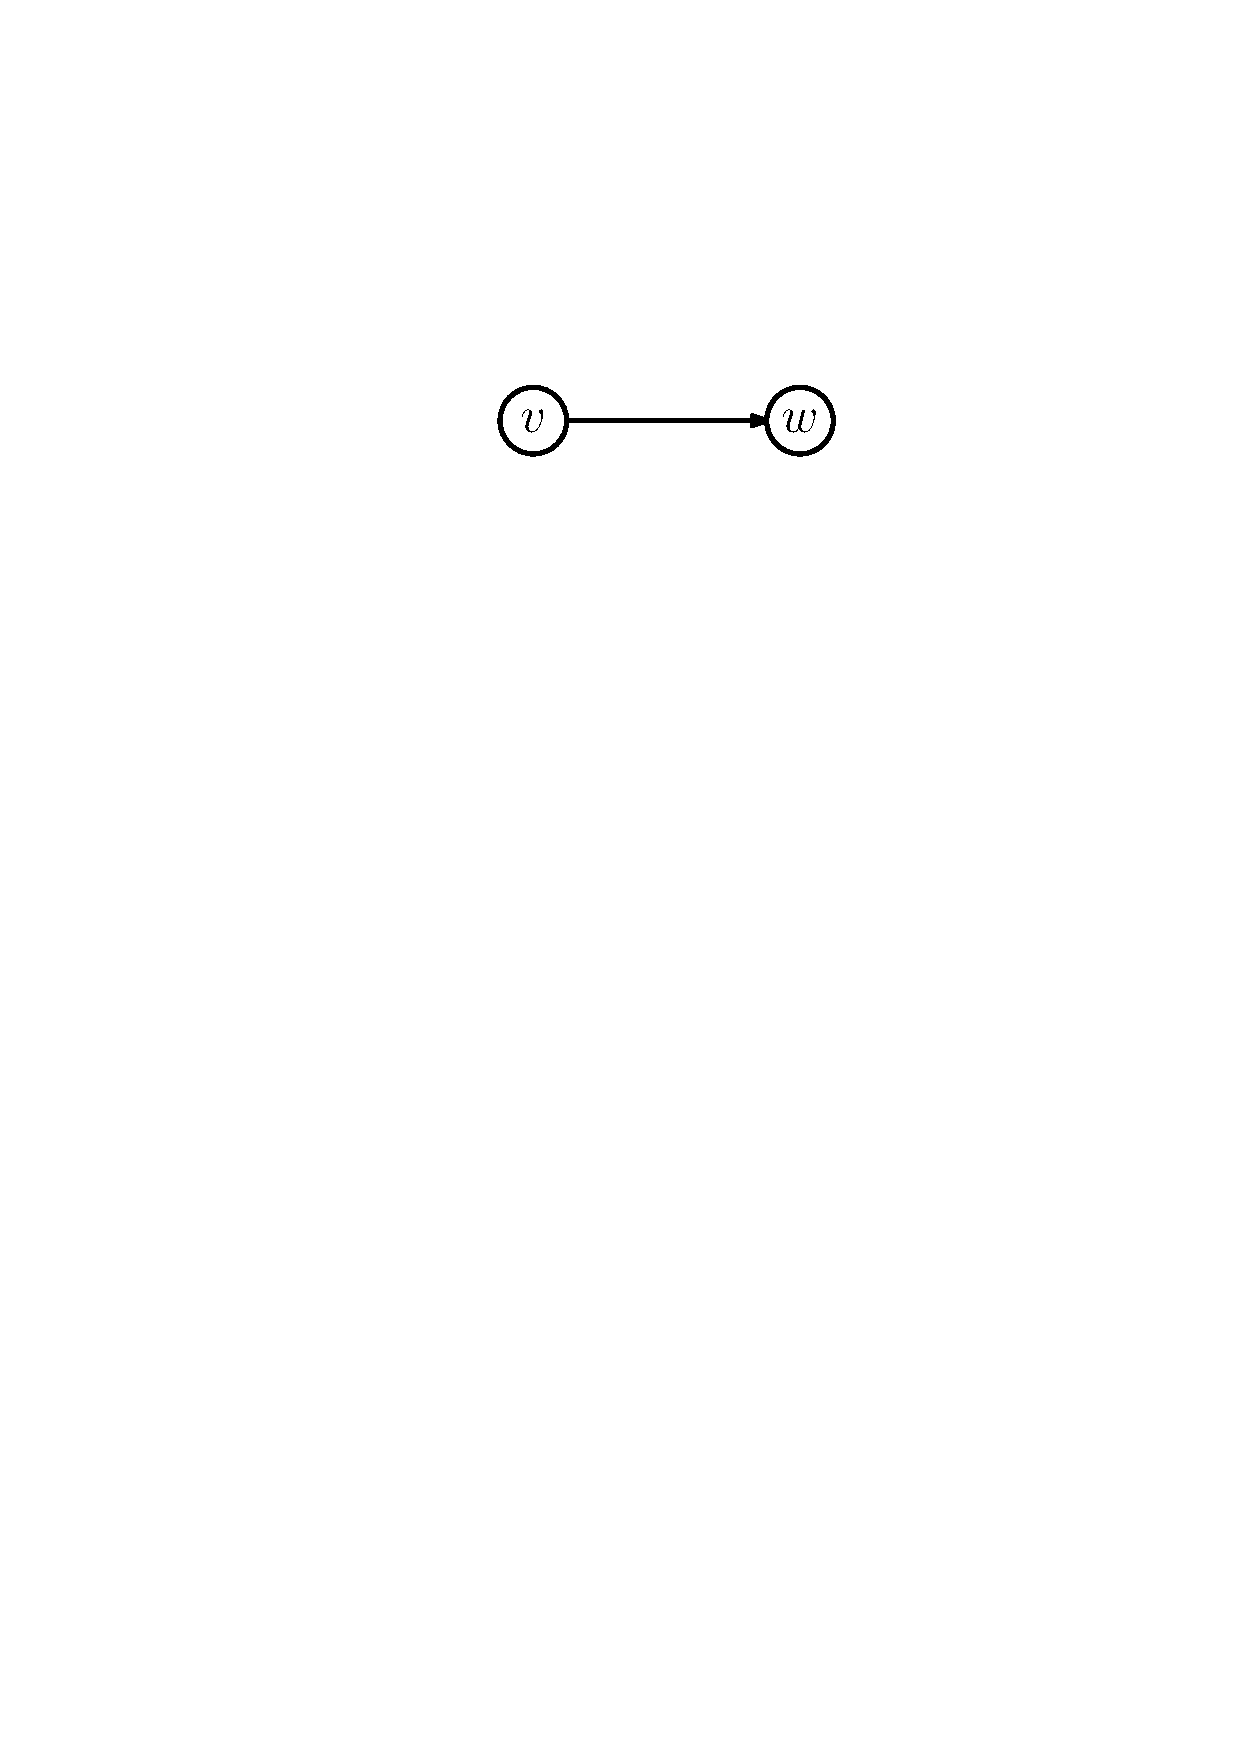
\includegraphics[scale=.5]{01_graph_theory/pics/directed-graph_edge.pdf}\\

undirected:& $ e = {v,w} = {w,v}, e = vw$\\
	& 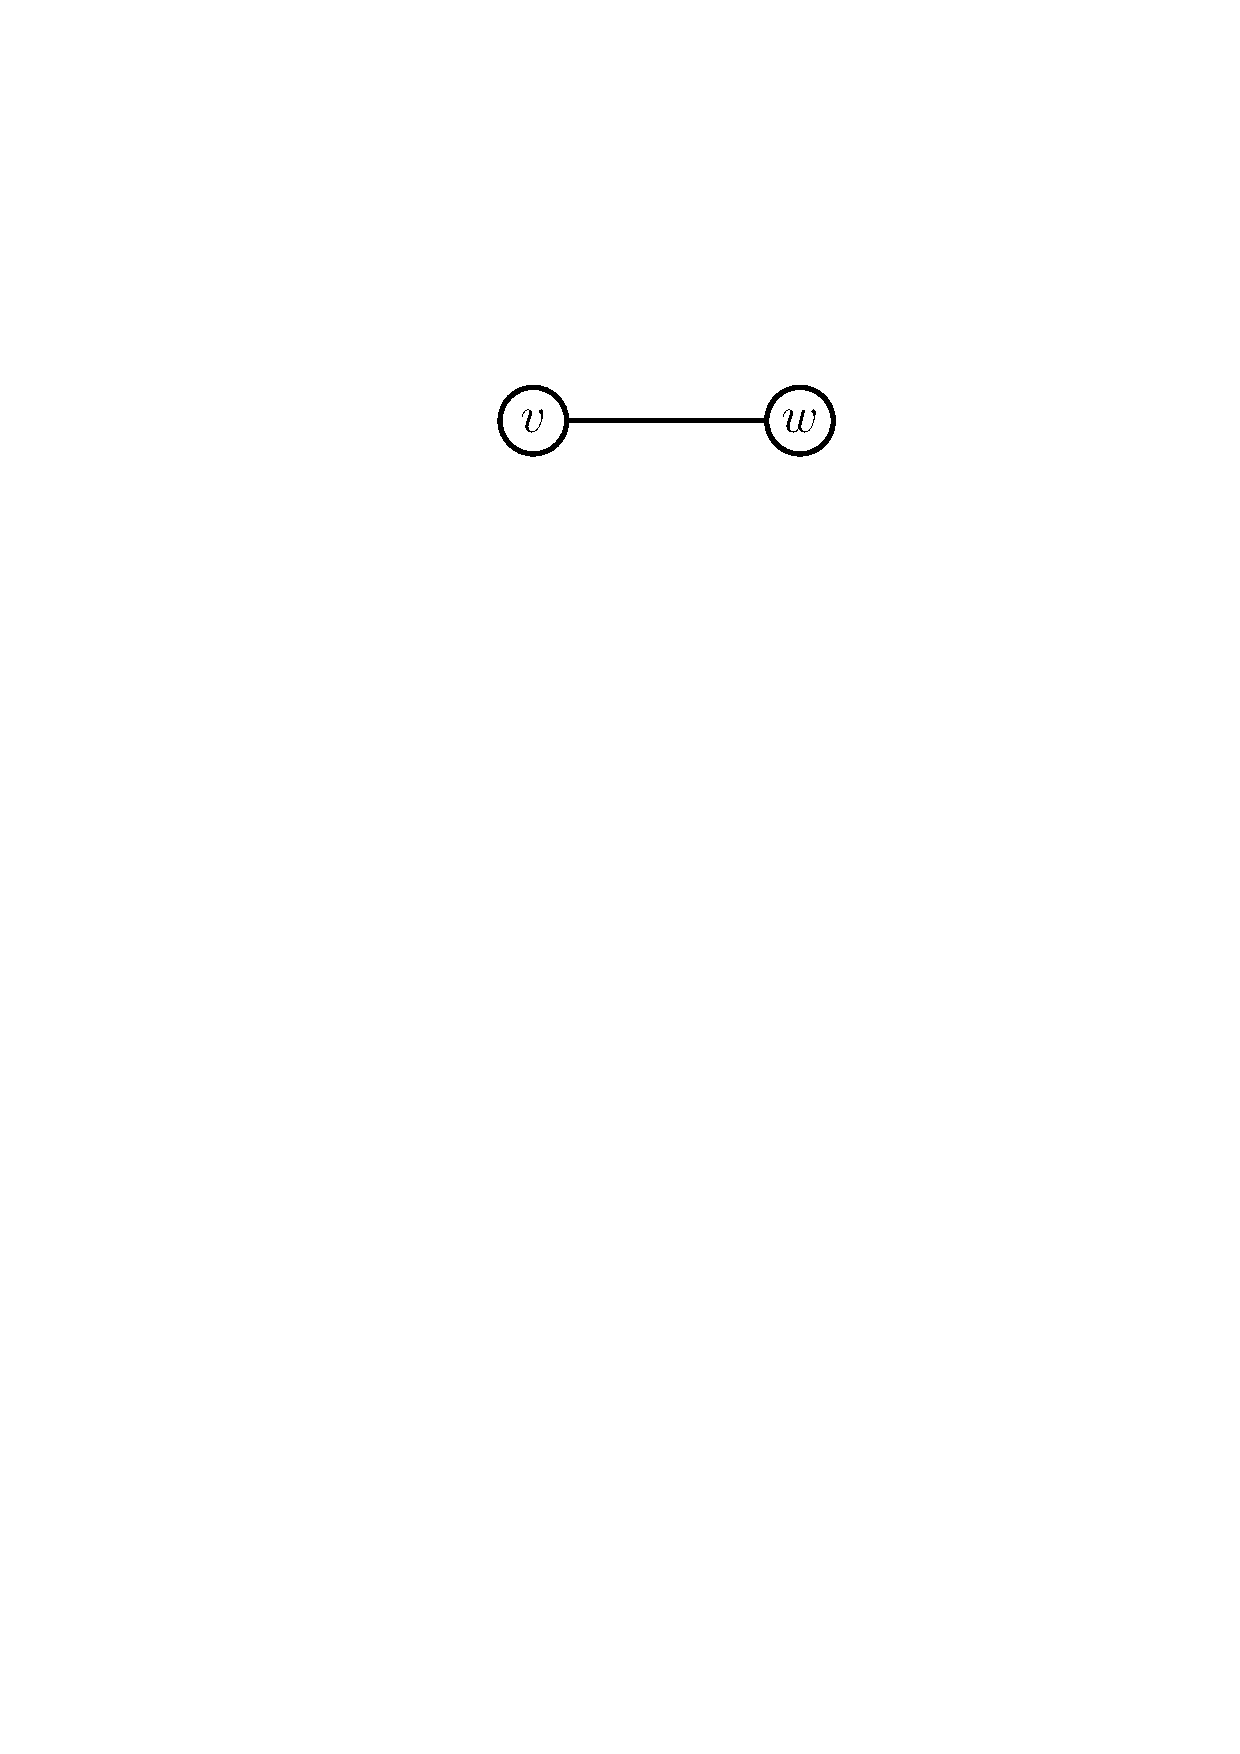
\includegraphics[scale=.5]{01_graph_theory/pics/graph_edge.pdf} \\

loop \\
	& 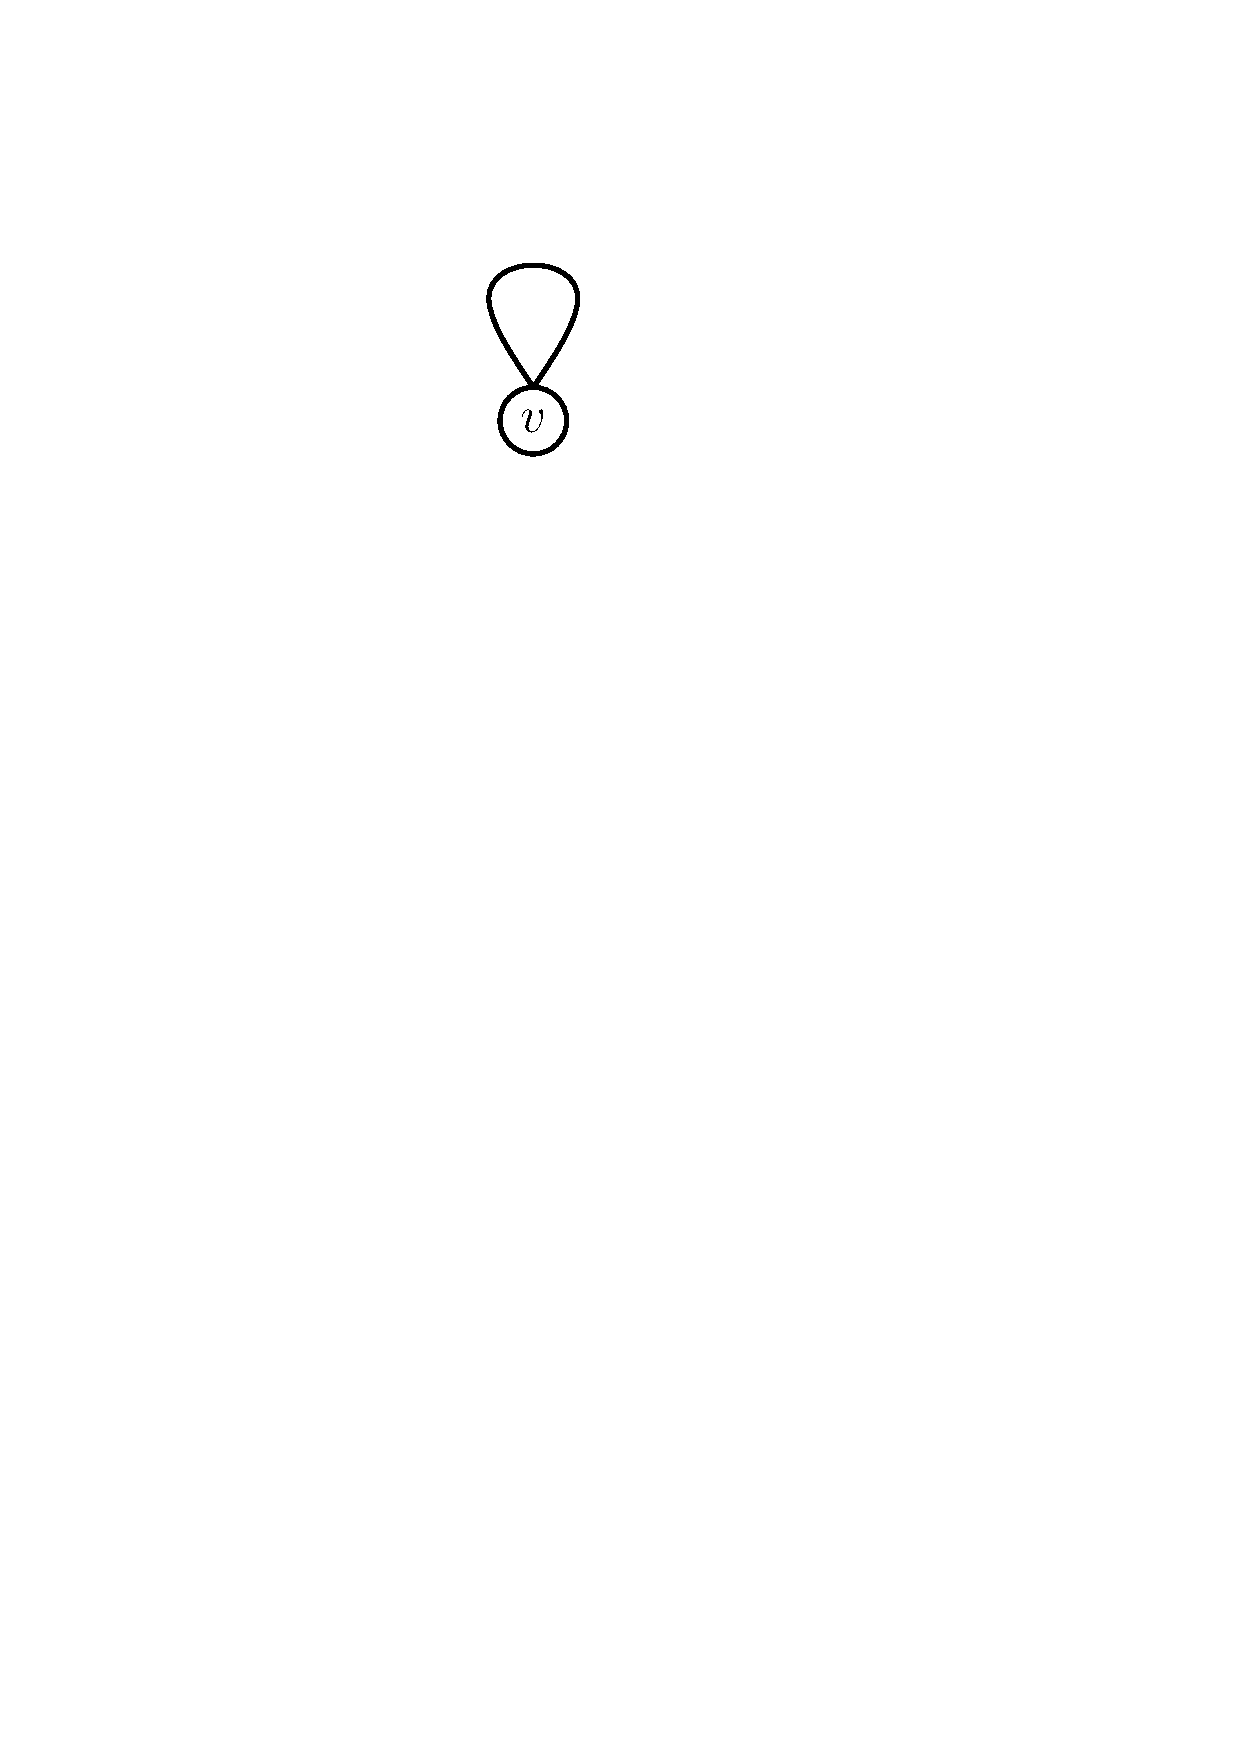
\includegraphics[scale=.5]{01_graph_theory/pics/graph_loop.pdf} \\

multiple Edges \\
	& 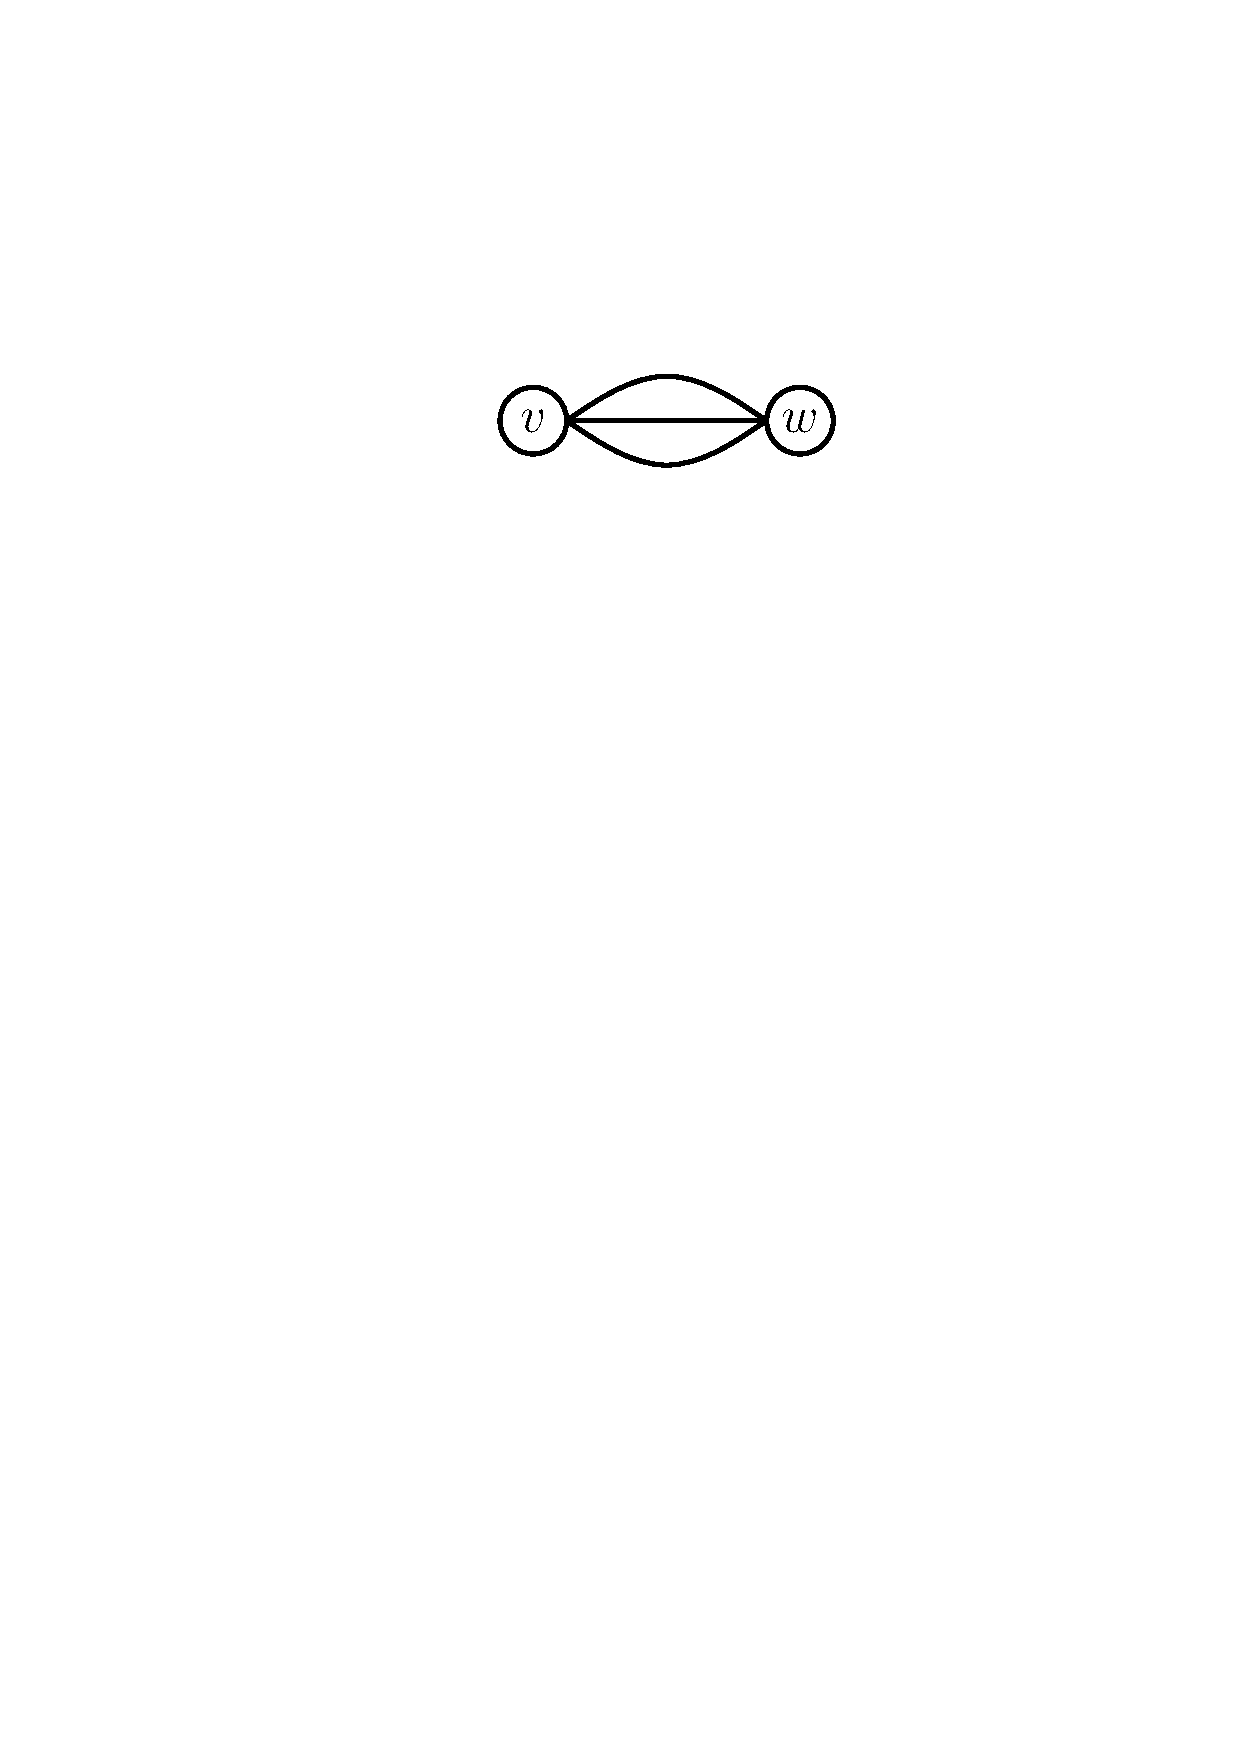
\includegraphics[scale=.5]{01_graph_theory/pics/graph_multiple-edges.pdf} \\


simple Graph: & if there are no loops, no multiple edges \\


\end{tabular}

graph corresponds to a relation on V $(\leq V \times V)$

unidirectional graph $\equiv$ symmetrix relation \\
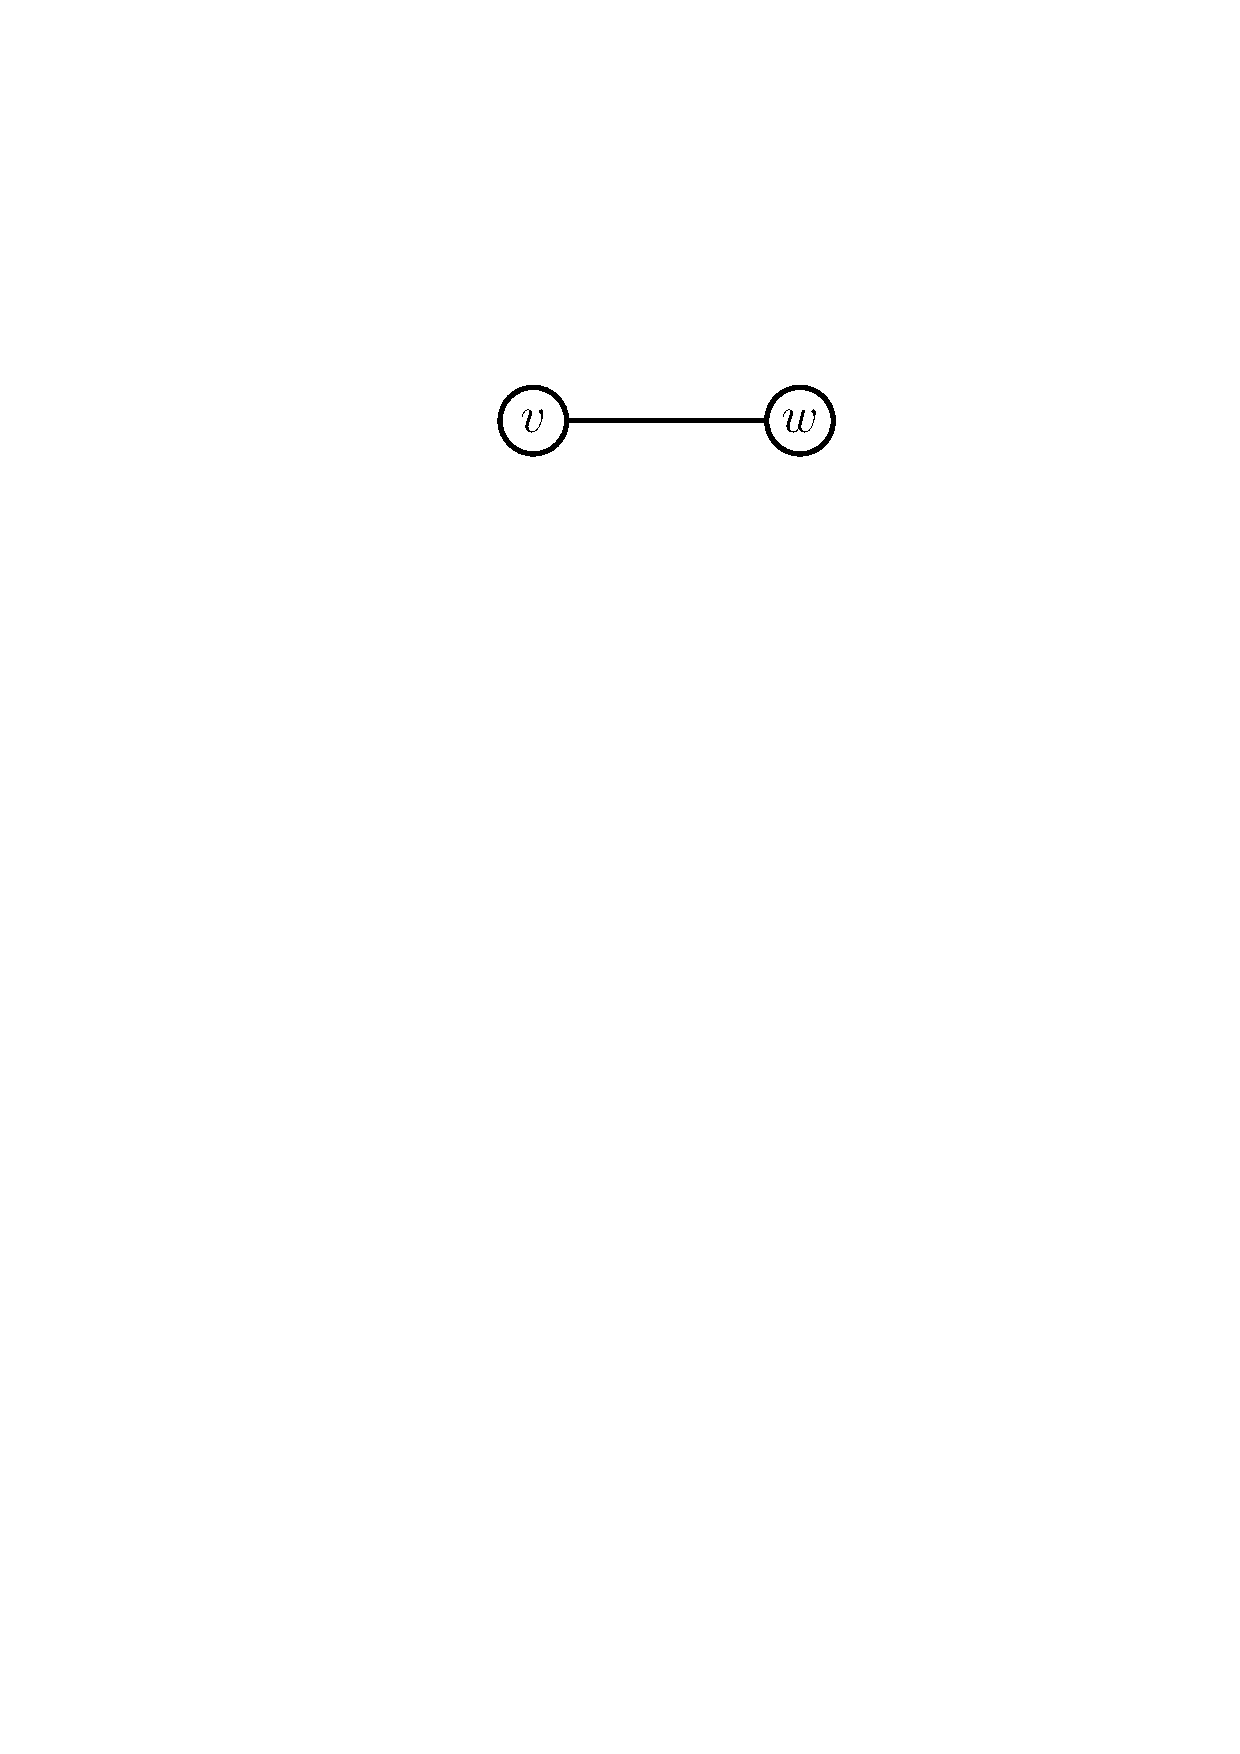
\includegraphics[scale=.5]{01_graph_theory/pics/graph_edge.pdf} $\equiv$ 
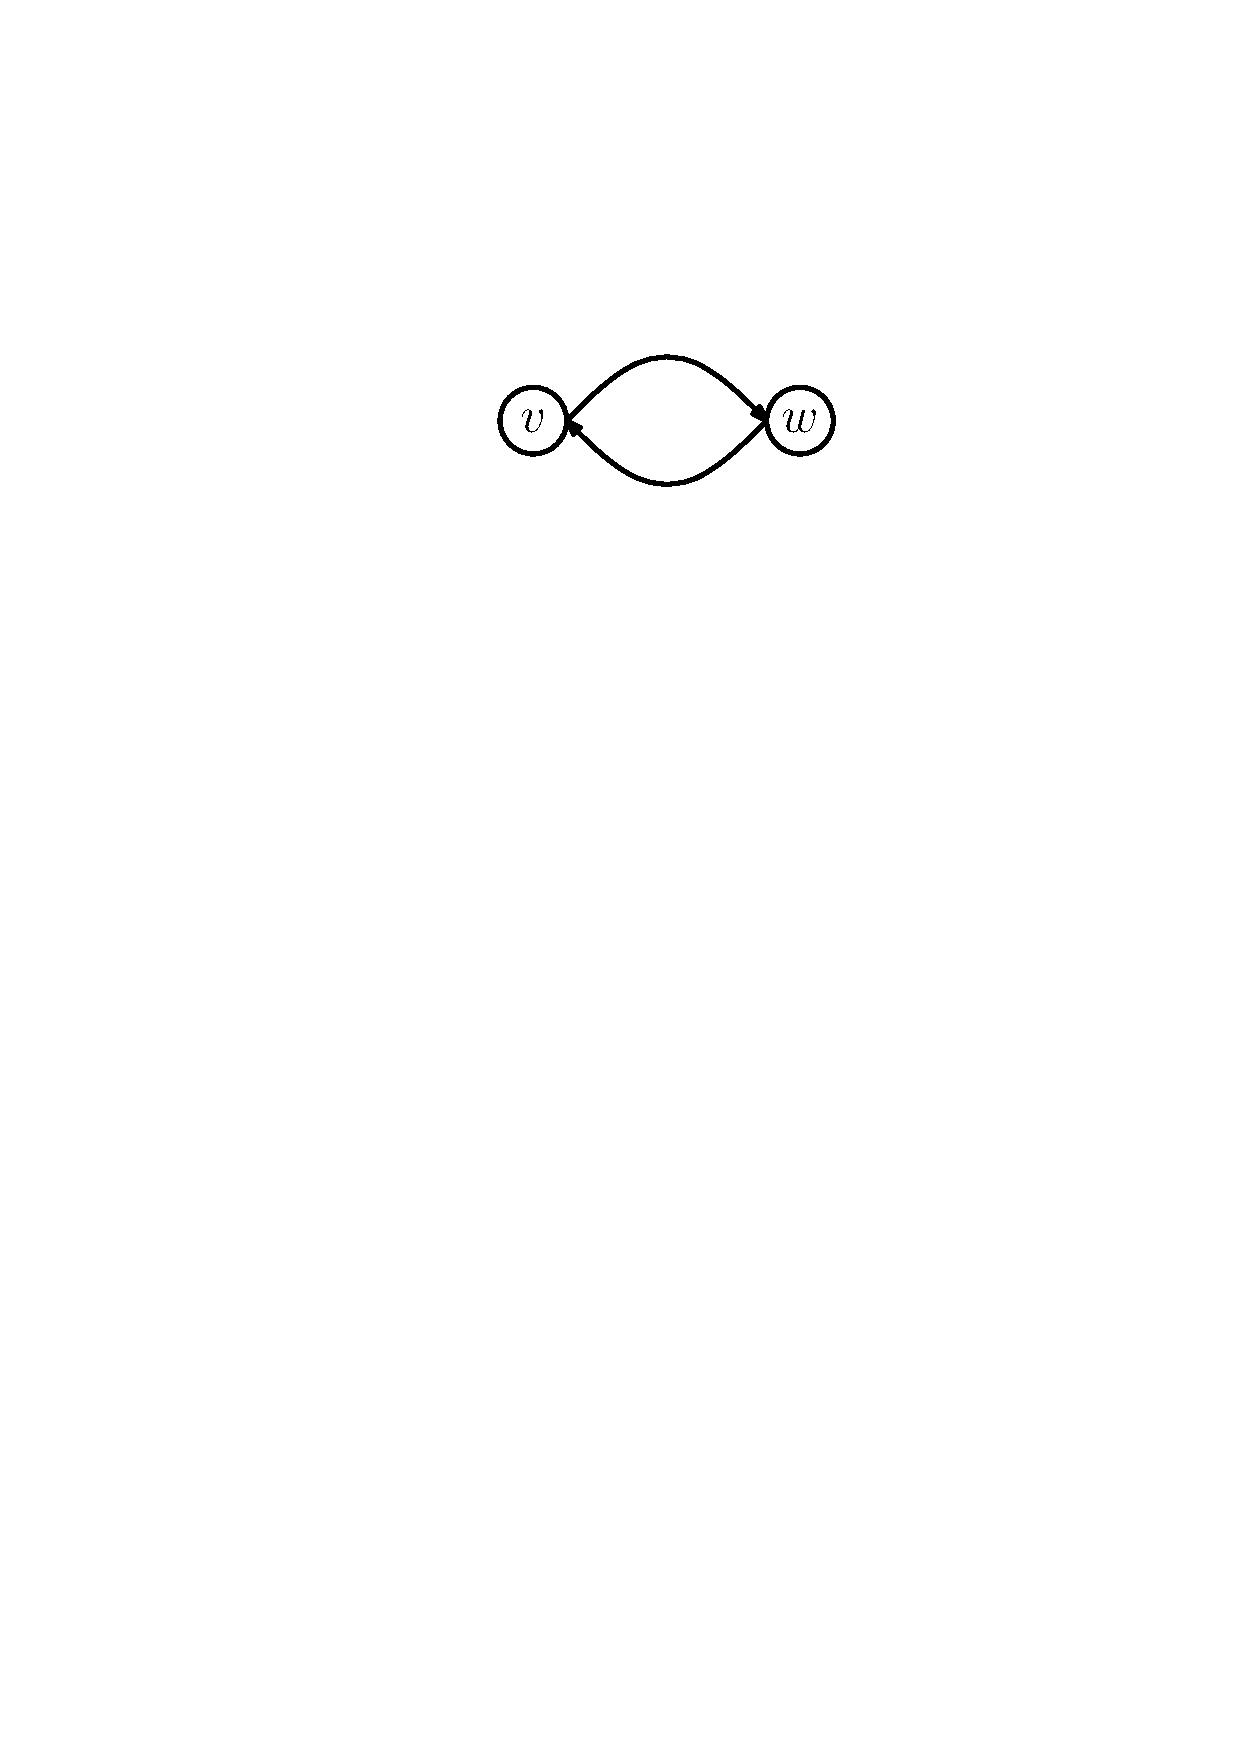
\includegraphics[scale=.5]{01_graph_theory/pics/directed-graph_multiple-edges.pdf} \\

\subsubsection*{Notations:}
$V = V(G), E = E(G), \alpha_0 = |V|, \alpha_1 = |E|$ 

\subsubsection*{Def:}

\begin{tabular}{l l}
$v \in V$ : \\
$d(v)$		& \# edges which are incident to v \\

$d^+(v)$	& \# edges of the form $(v,w)$, out degree \\
$d^-(v)$	& \# edges of the form $(w,v)$, in degree \\

$\Gamma(v)$ & set of neighbours \\
$\Gamma^+(v)$ & set of successors \\
$\Gamma^-(v)$ & set of predecessors \\

\end{tabular}

\begin{figure}[htb]
\centering
\subfigure[vertex $v$ with degree $d(v)=6$]{
	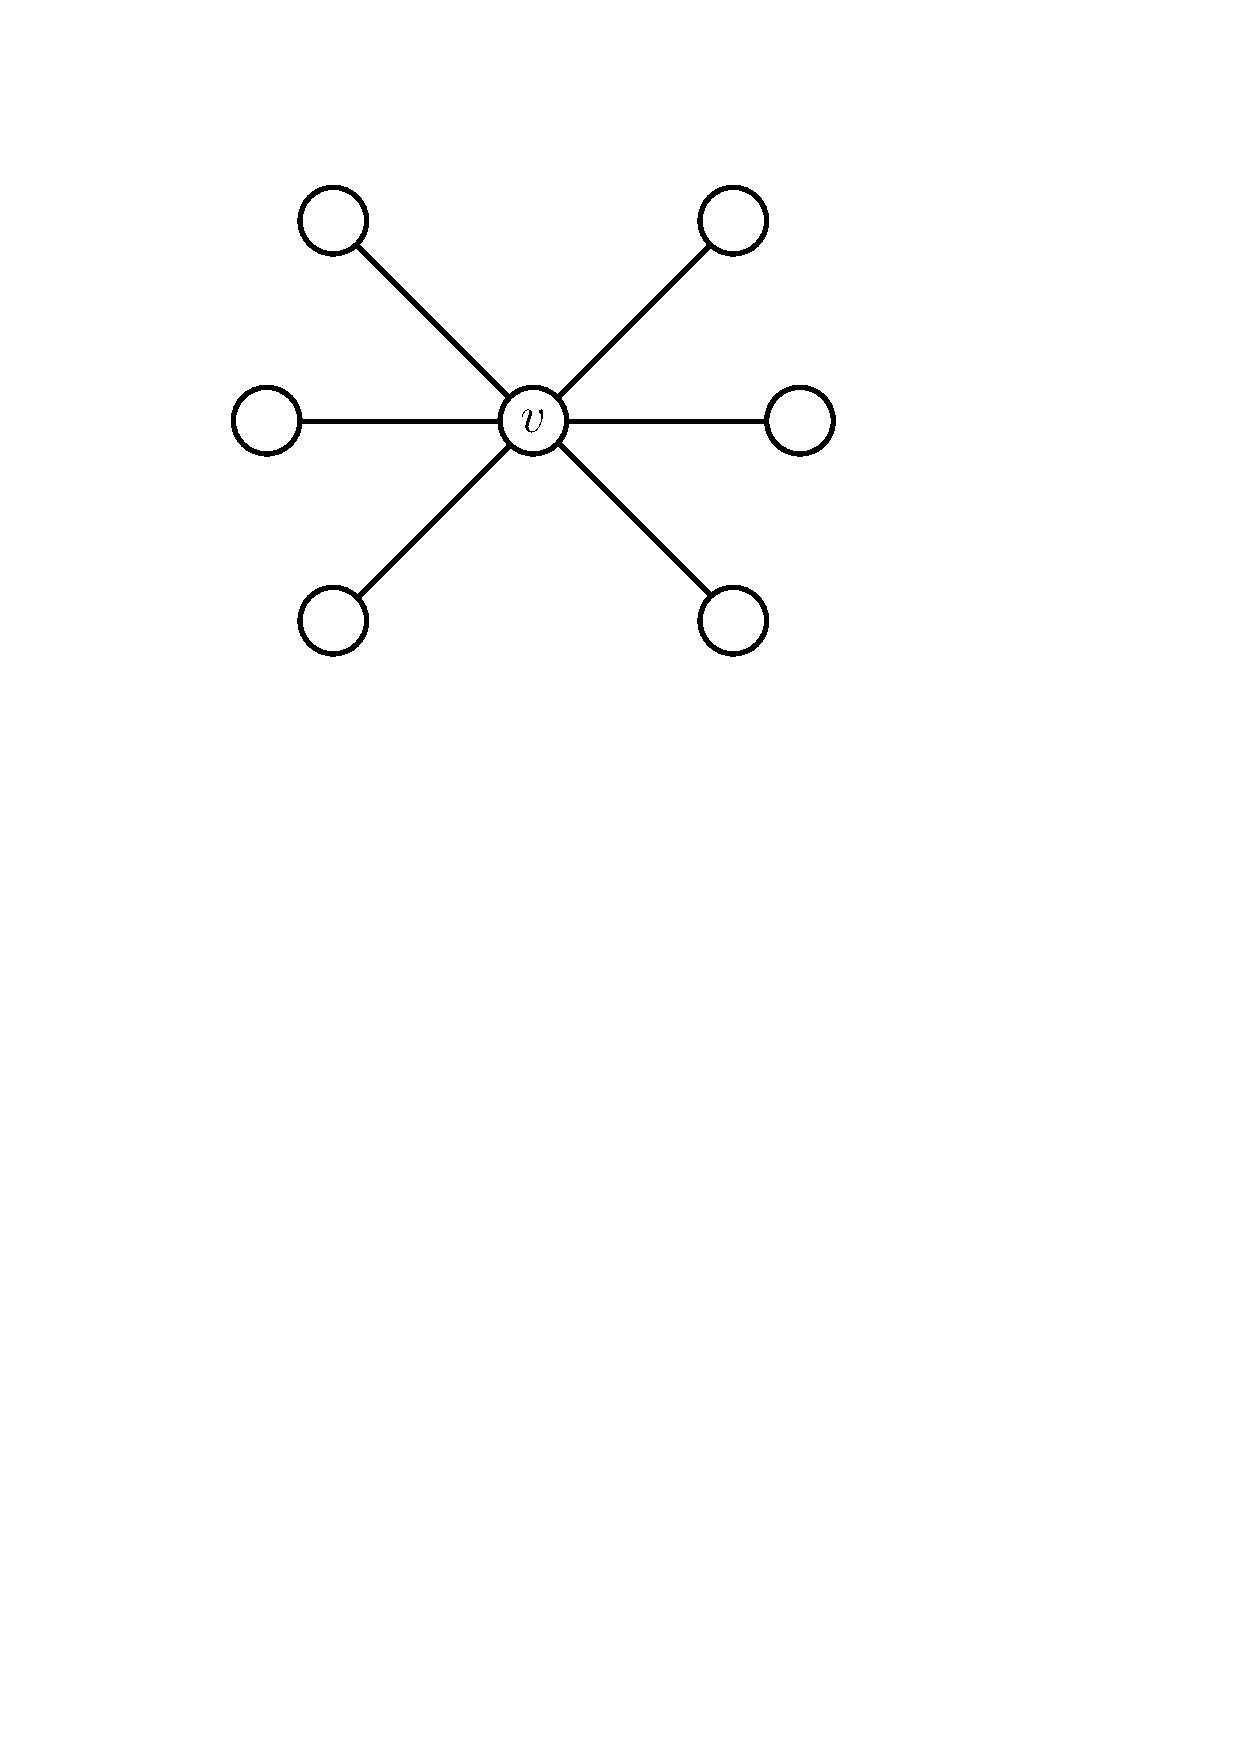
\includegraphics[scale=.5]{01_graph_theory/pics/graph_degree.pdf}
}
\subfigure[vertex $v$ with in-degree $d^{-}(v)=3$ and out-degree $d^{+}(v)=3$]{
	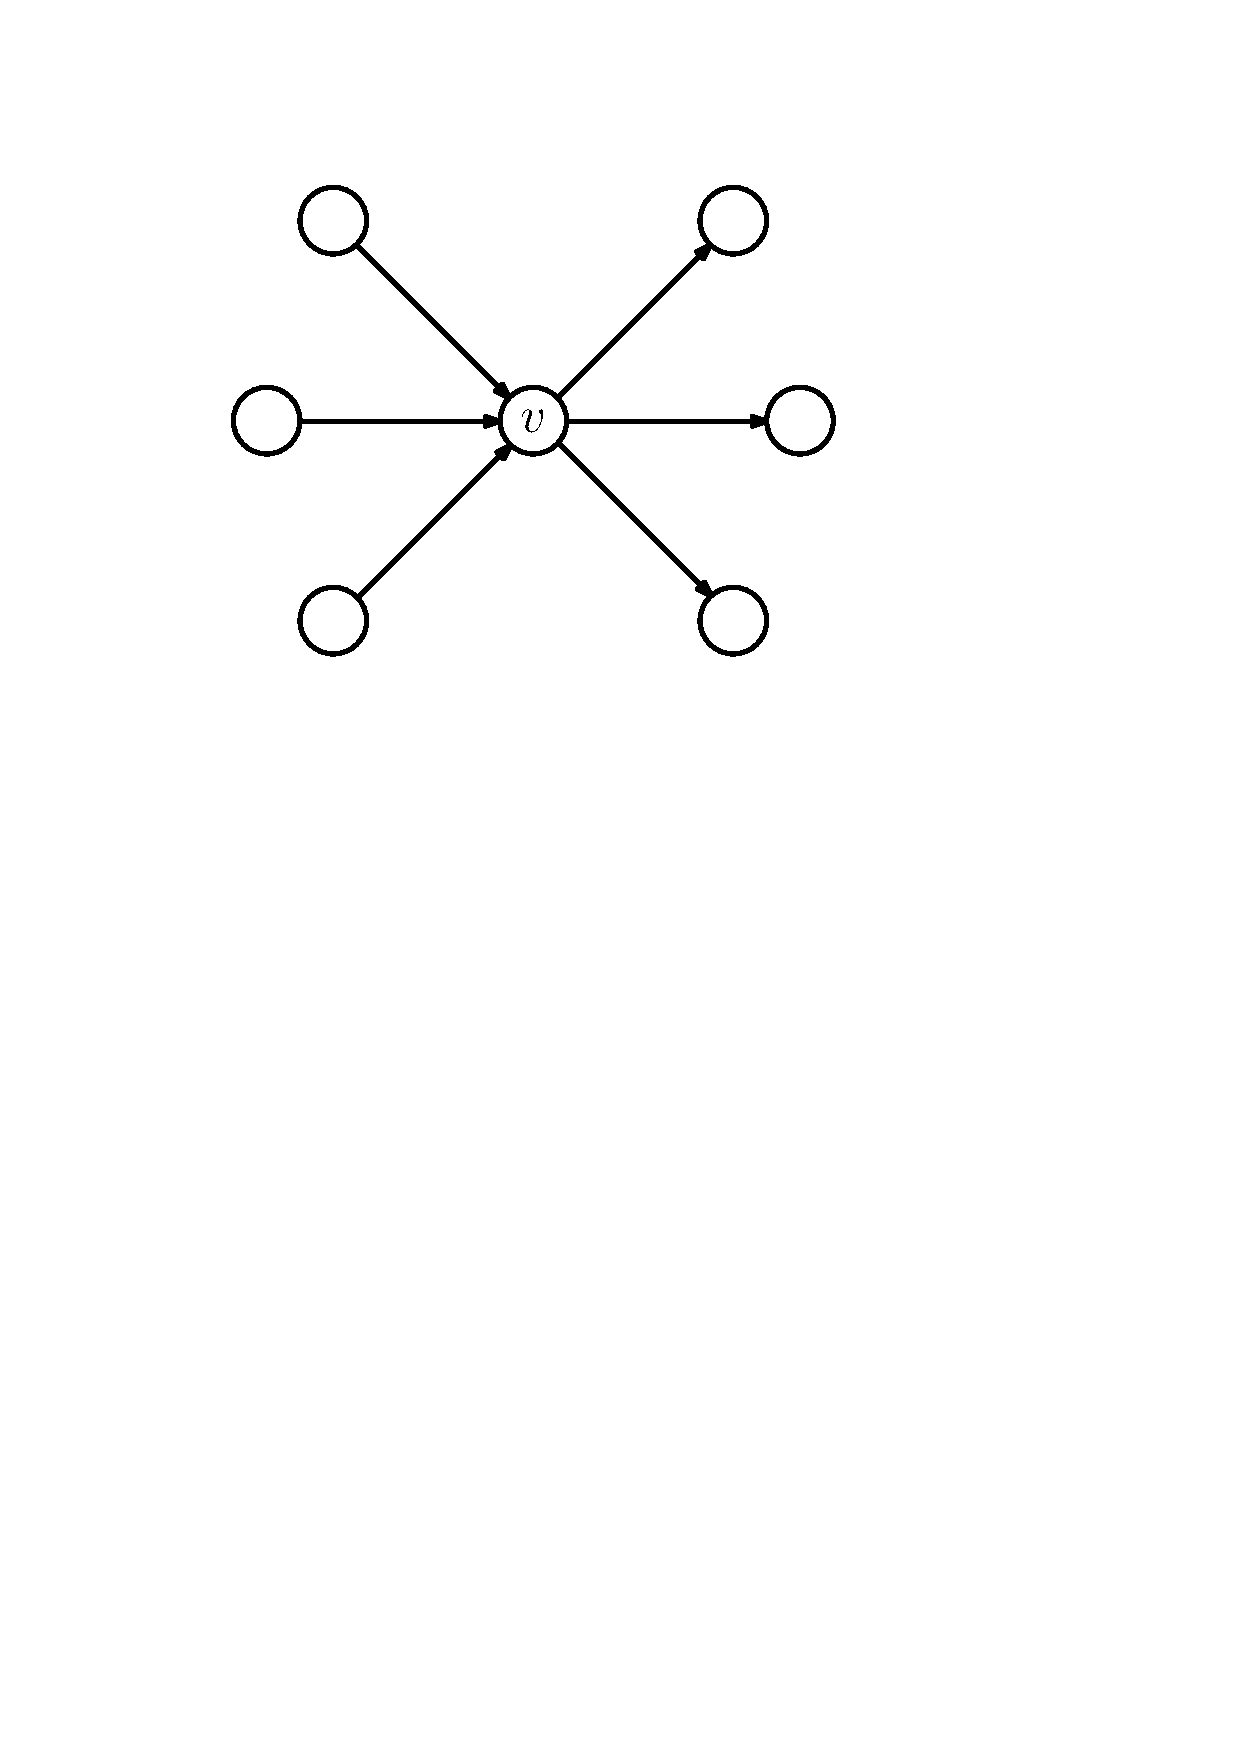
\includegraphics[scale=.5]{01_graph_theory/pics/directed-graph_indegree-outdegree.pdf}
}
\caption{vertex-degrees}
\end{figure}
\FloatBarrier

\subsubsection*{Hand Shaking Lemma (simple graphs)}
$\sum_{v \in V} d(v) = 2 |E|$\\
$\sum_{v \in V} d^+(v) = d^-(v) = |E|$

\begin{figure}[htb]
\centering
\subfigure[undirected graph, each edge is counted twice]{
	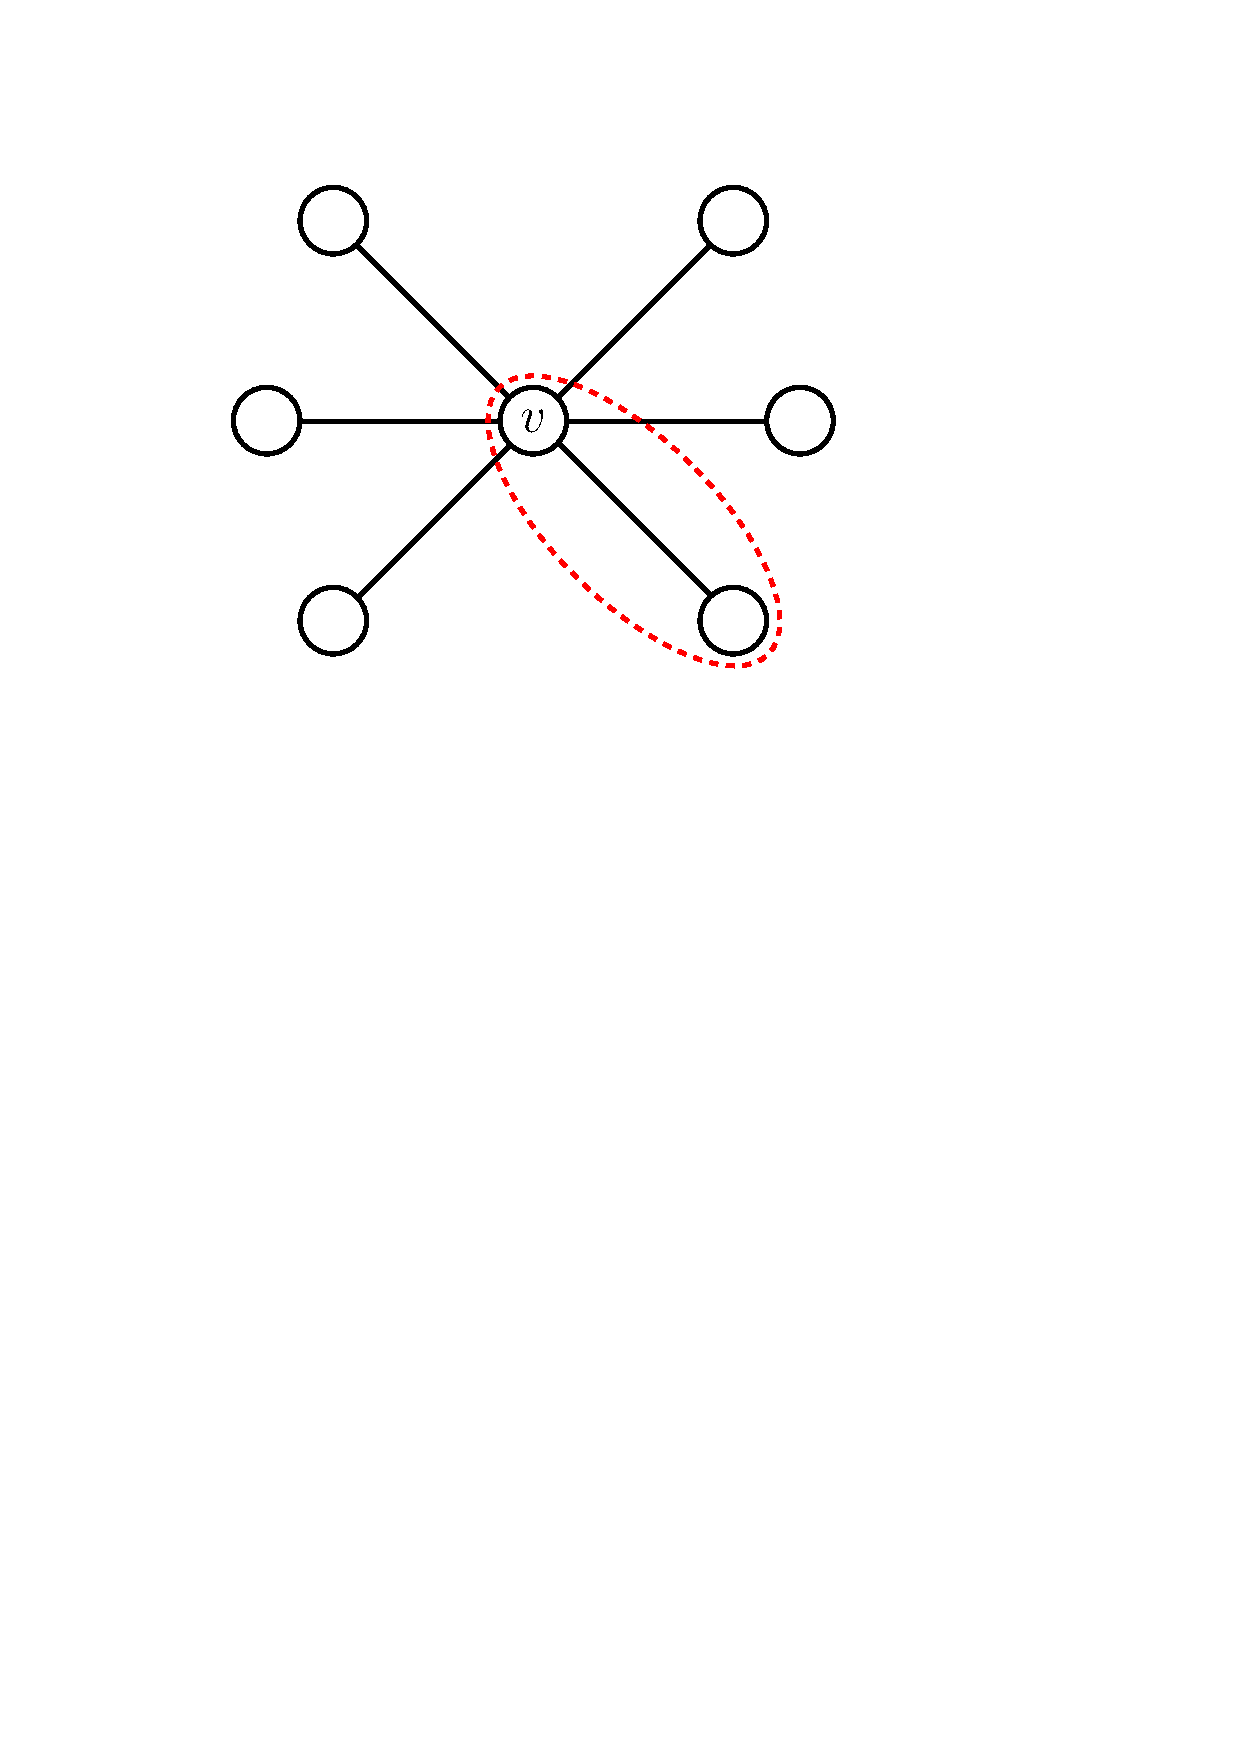
\includegraphics[scale=.5]{01_graph_theory/pics/graph_degree_handshaking-lemma.pdf}
}
\subfigure[directed graph, each edge is counted only once]{
	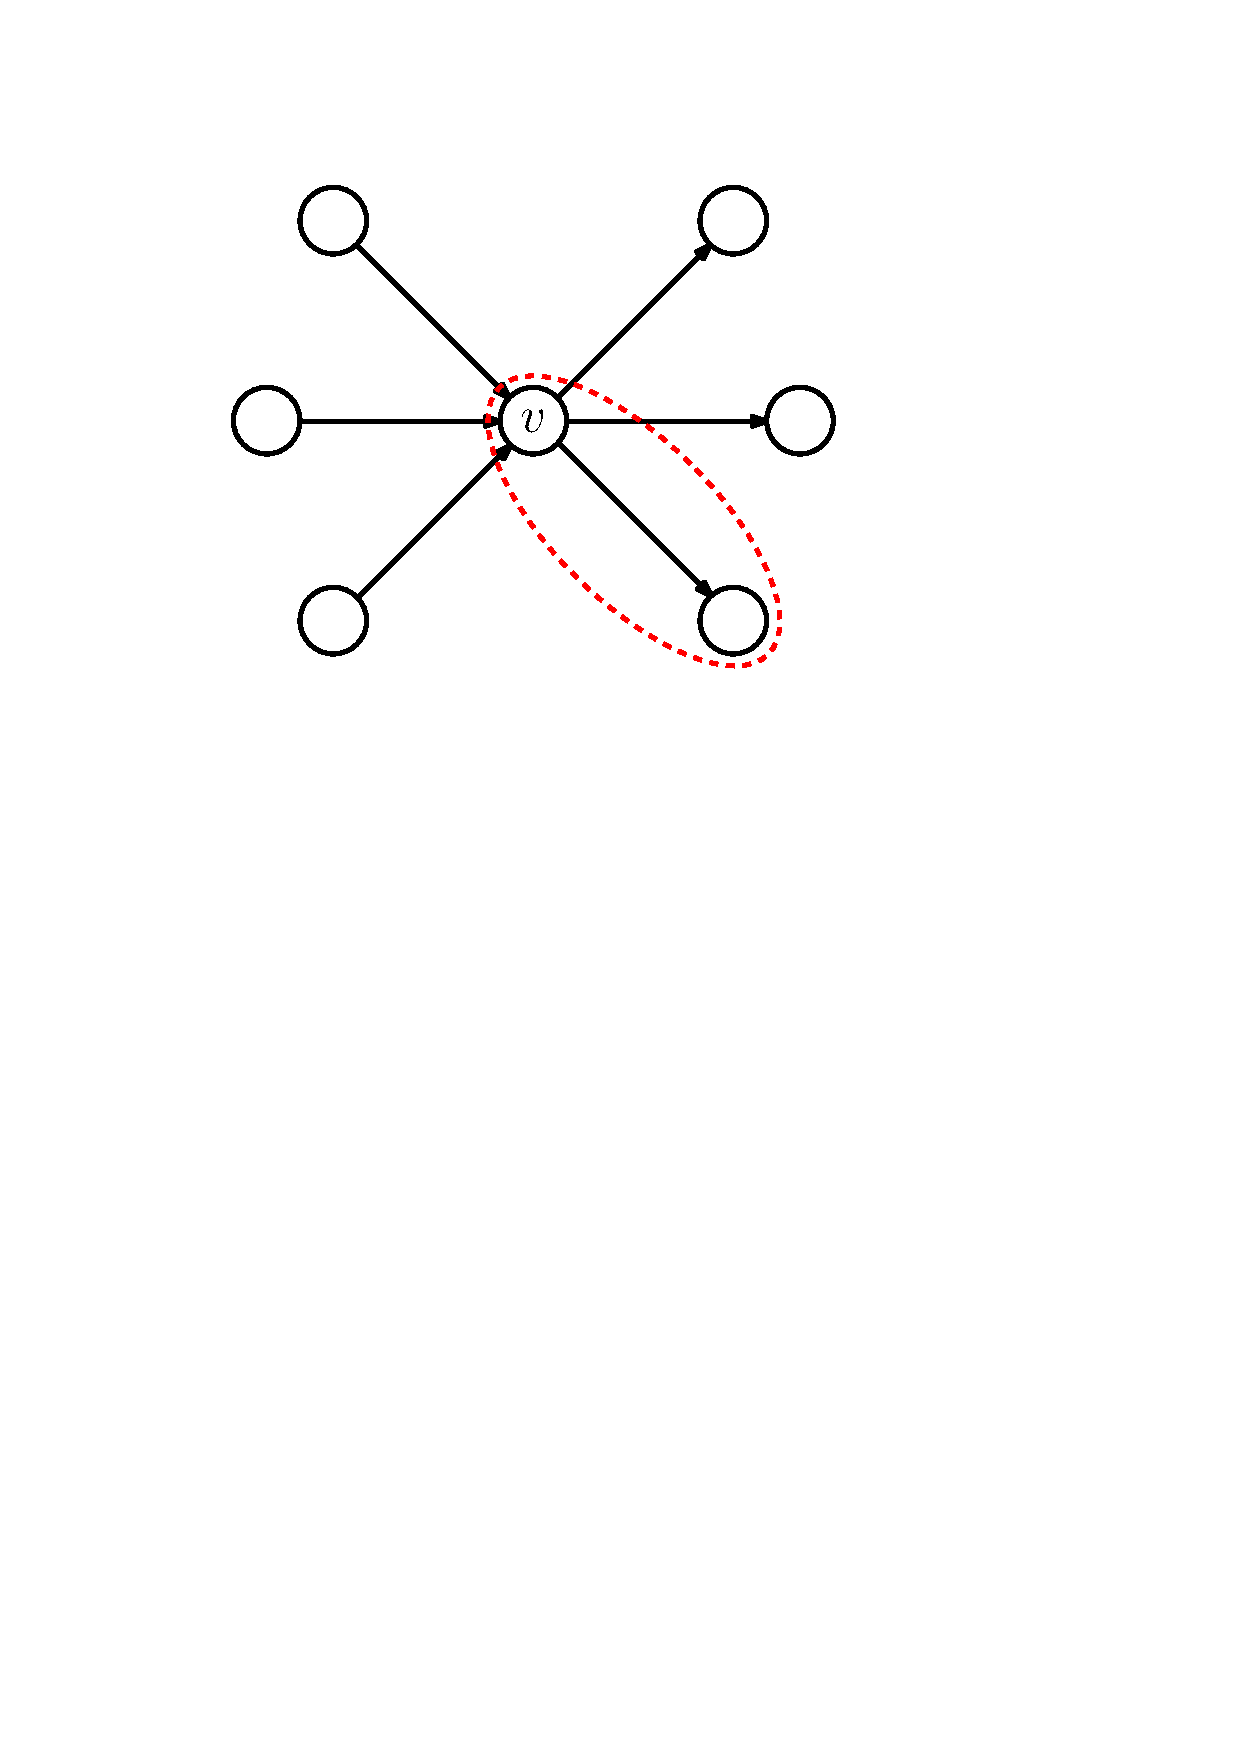
\includegraphics[scale=.5]{01_graph_theory/pics/directed-graph_degree_handshaking-lemma.pdf}
}
\caption{Hand Shaking Lemma in undirected and directed graphs}
\end{figure}
\FloatBarrier

\subsubsection*{Example: n-Hypercube:}
$G = ({0,1}^n, E)$

$vw \in E \Leftrightarrow \sum_{i=1}^{n} |v_i - w_i | = 1$ (only one switch in coordinates)

$v = v_1, v_2, \ldots , v_n$\\
$w = w_1, w_2, \ldots , w_n$

compute $a_0$ and $a_1$

$a_0 = 2^n$ \\
$a_1 = \frac{1}{2} \sum_{v \in V} d(v) = 2^{n-1} * n$

$d(v) = n \Rightarrow $ regular Graph
\begin{figure}[htb]
\centering
\subfigure[1D-hypercube]{
	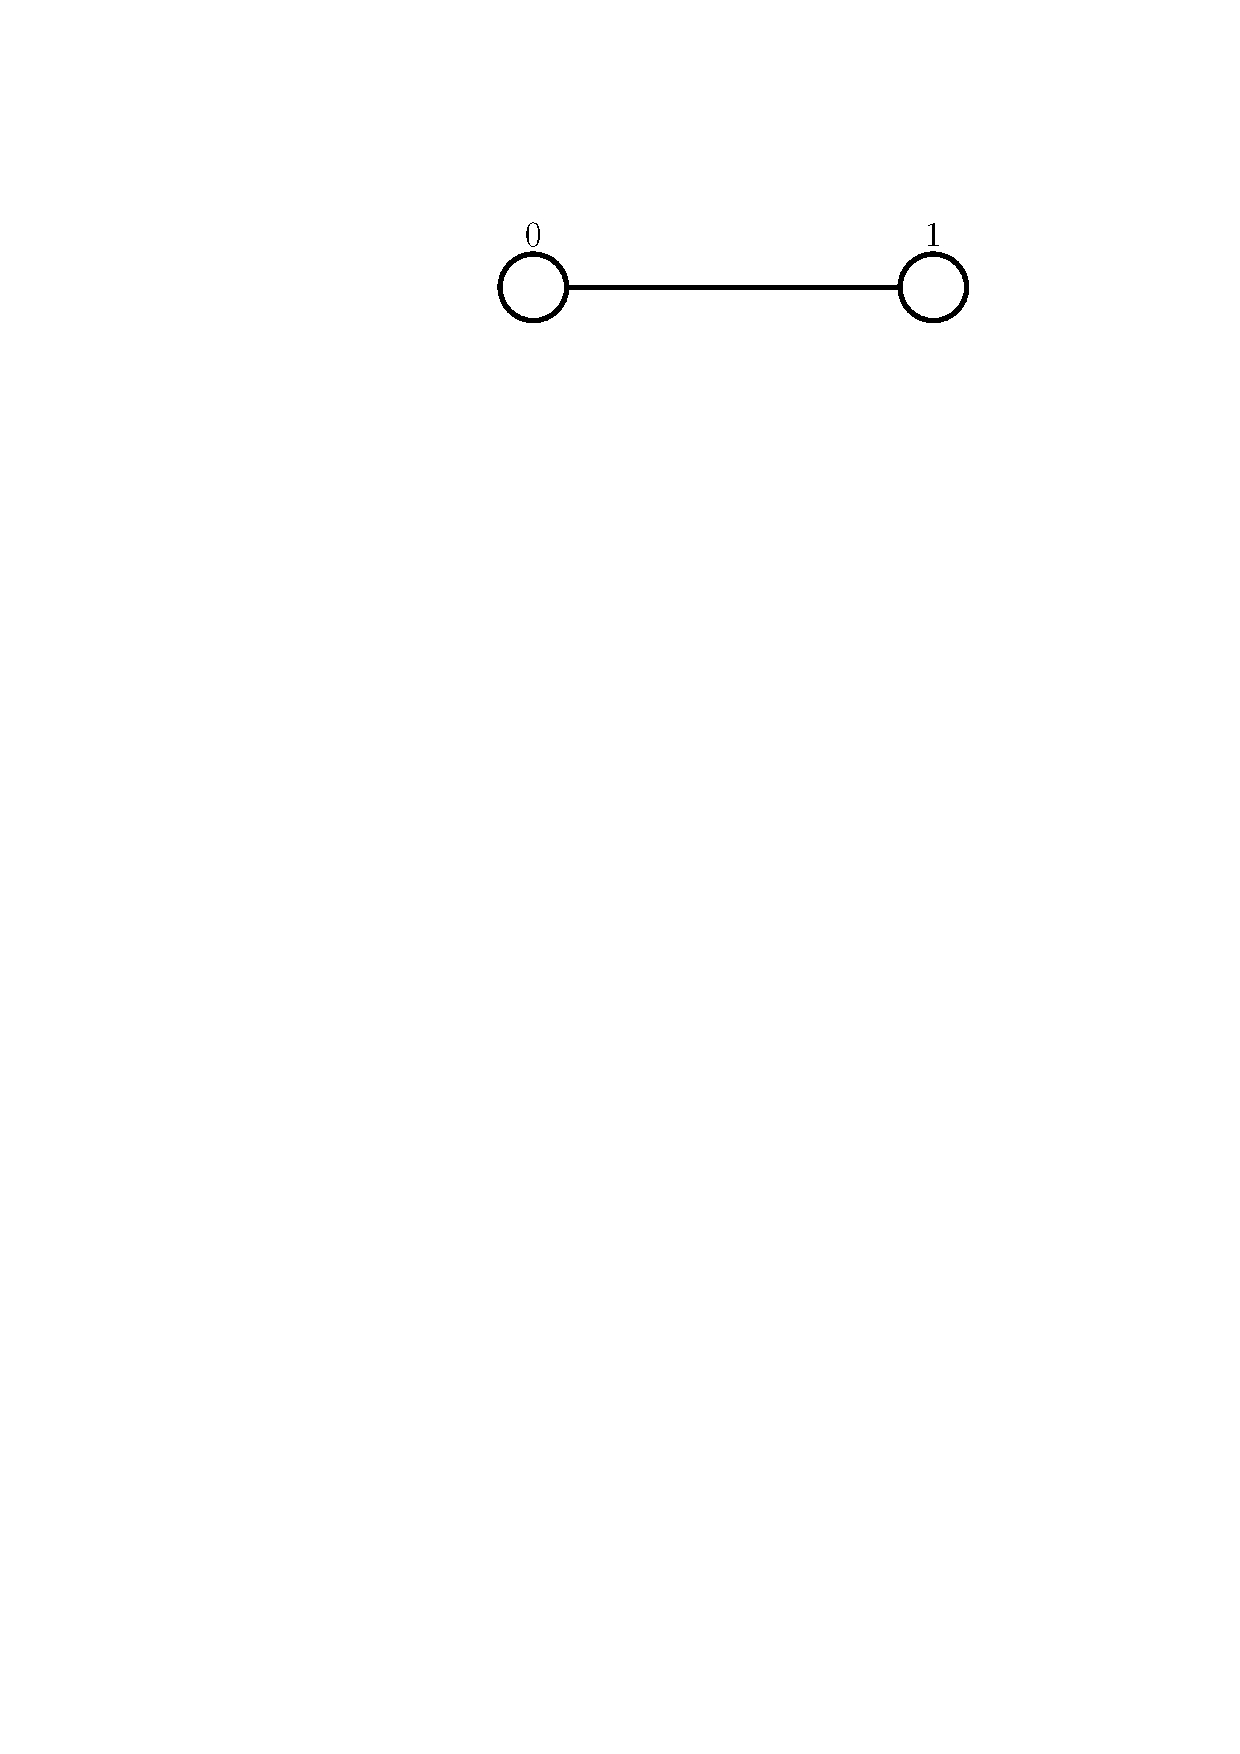
\includegraphics[scale=.4]{01_graph_theory/pics/1D-cube.pdf}
}
\subfigure[2D-hypercube]{
	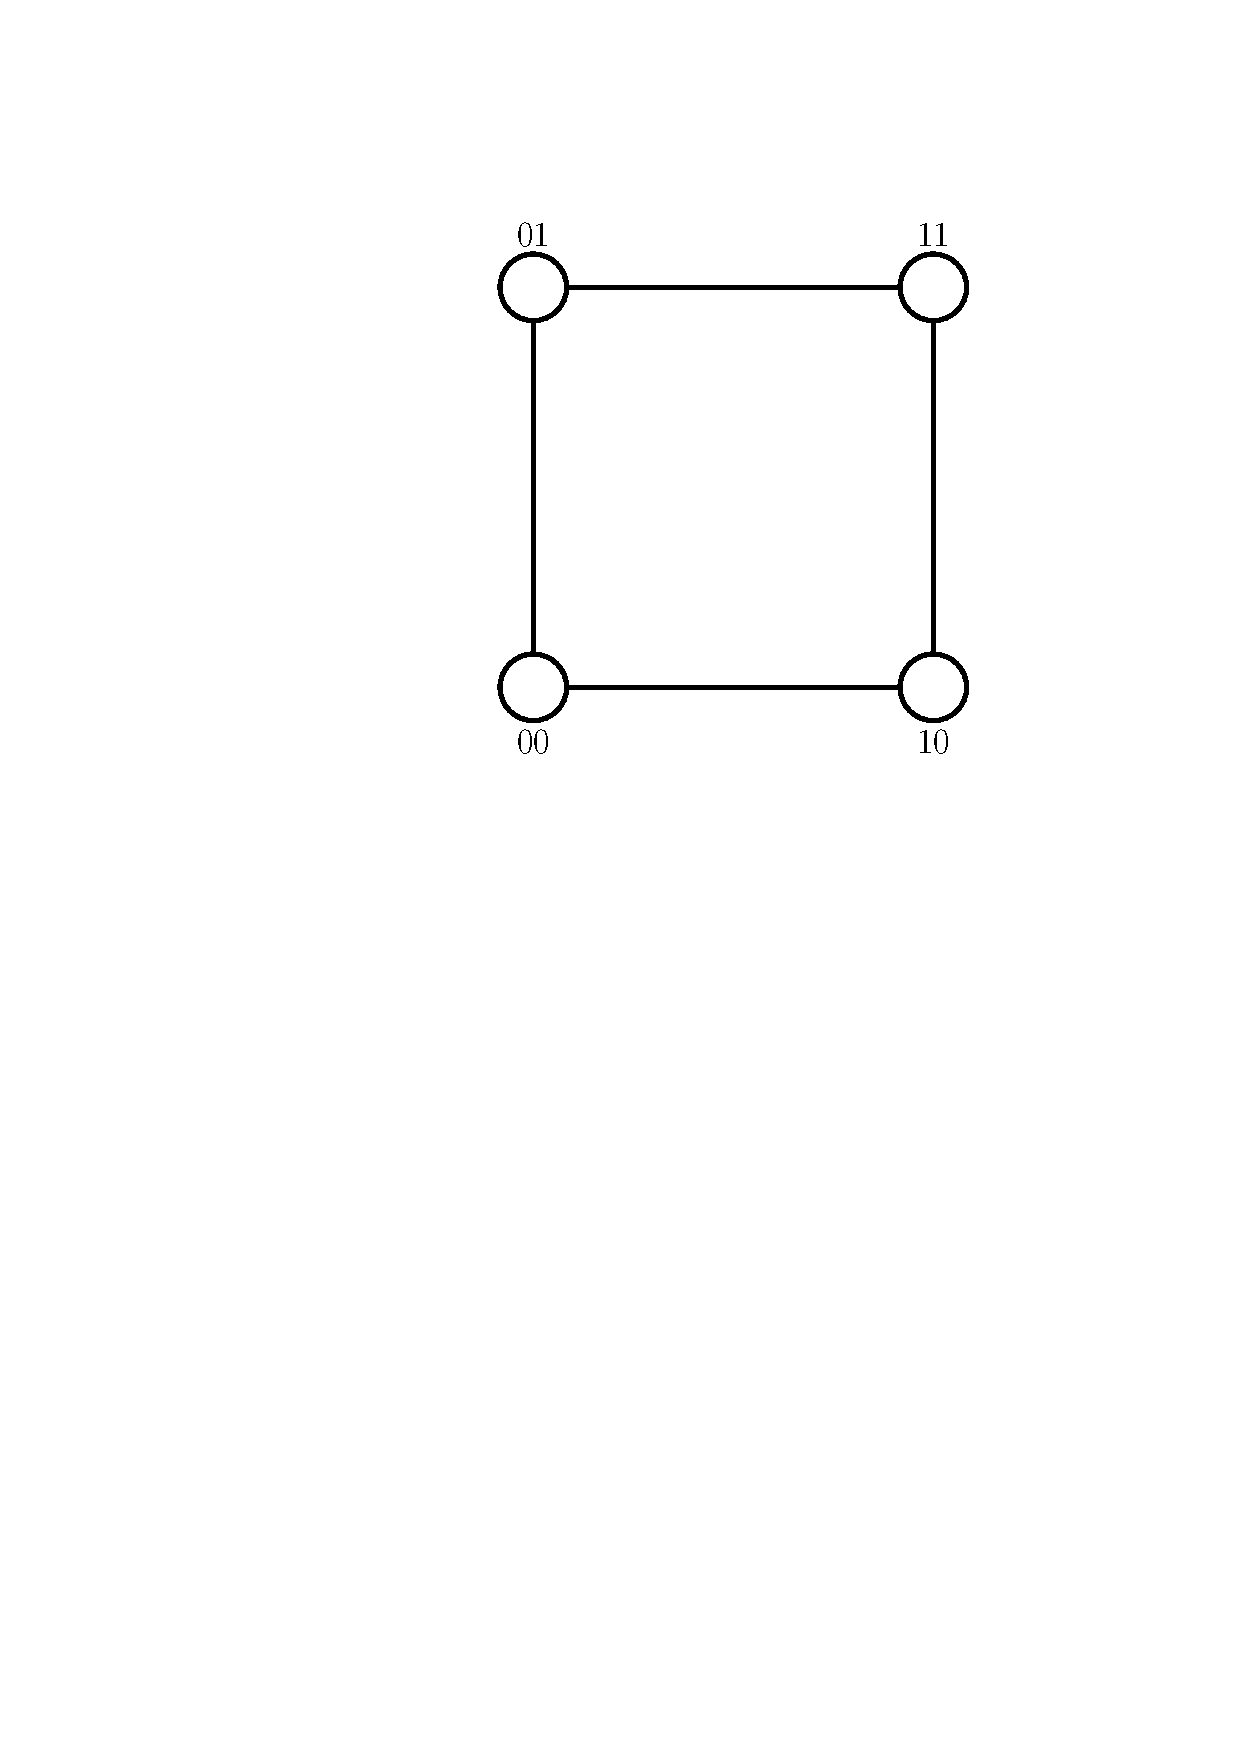
\includegraphics[scale=.4]{01_graph_theory/pics/2D-cube.pdf}
}
\subfigure[3D-hypercube]{
	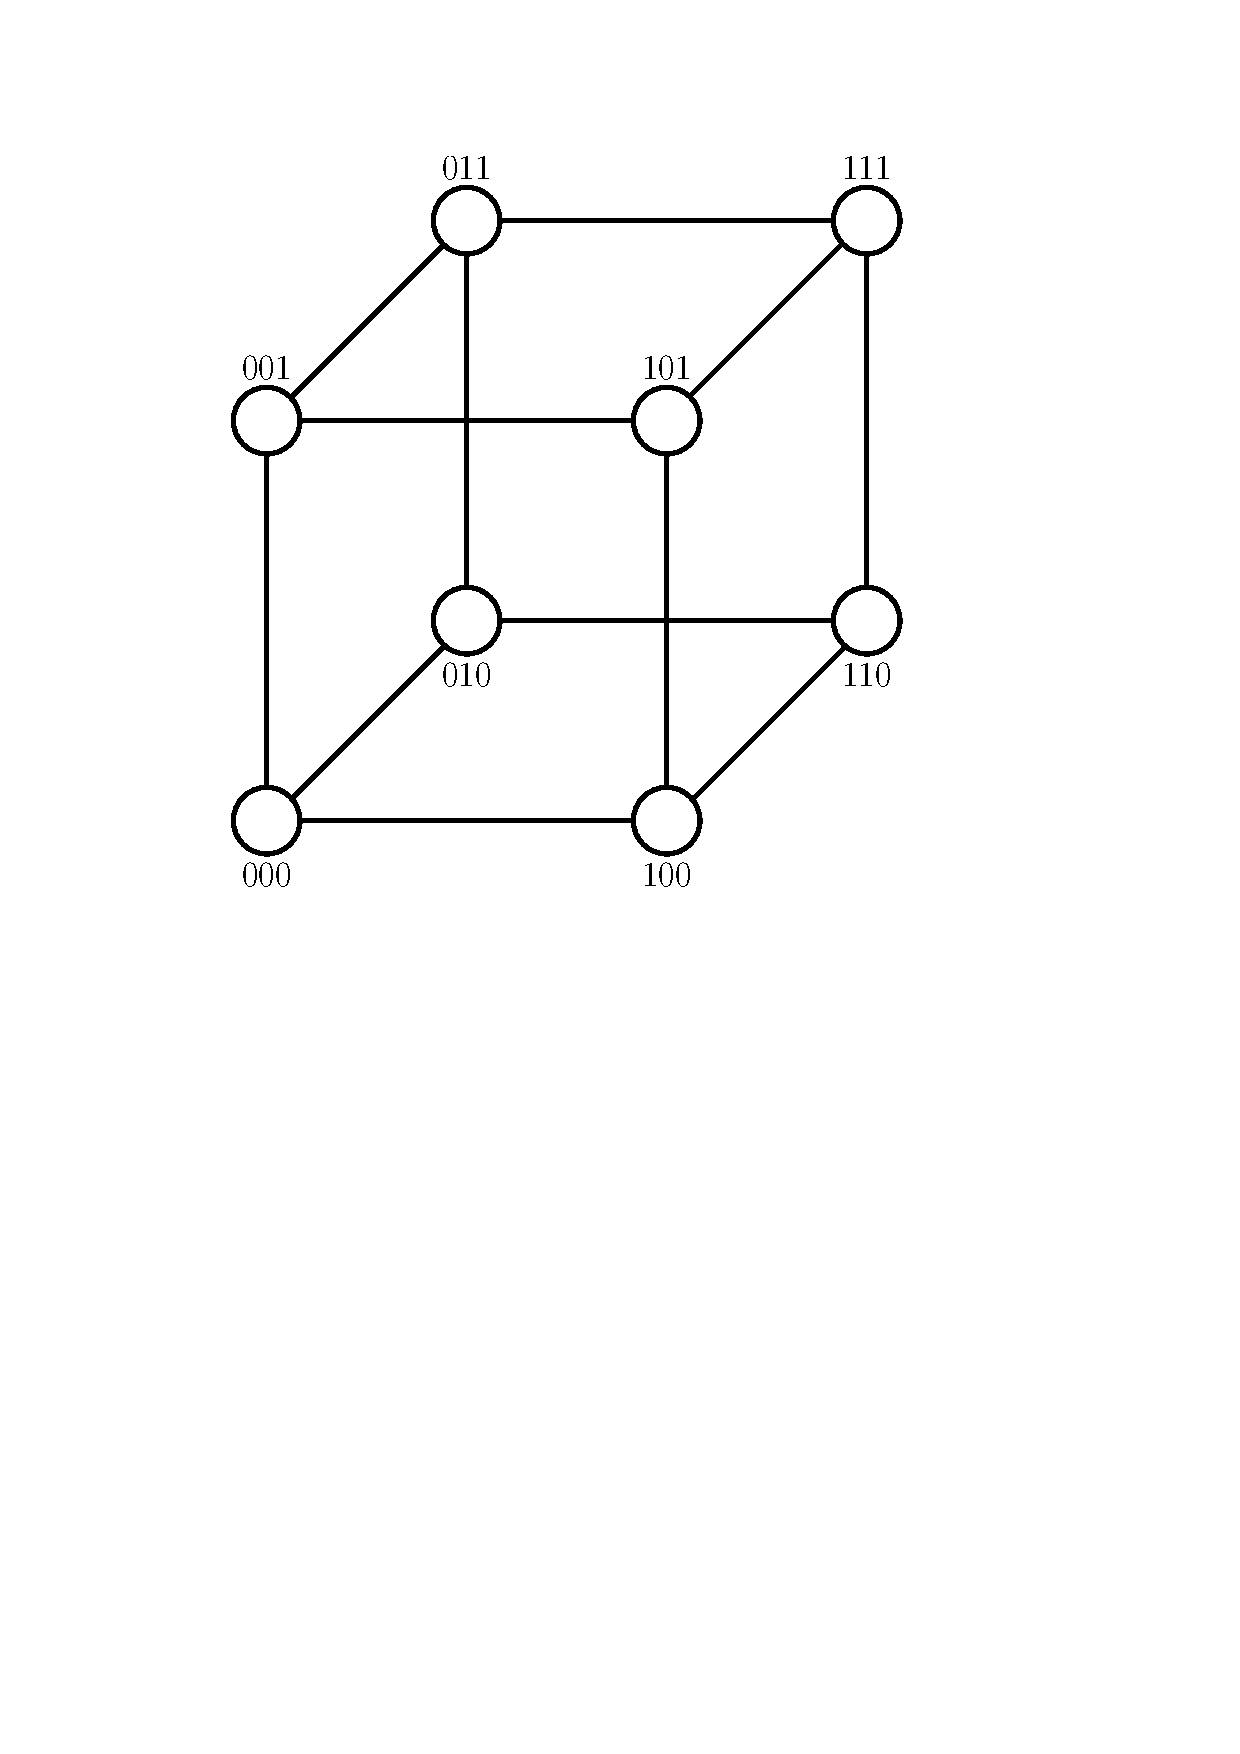
\includegraphics[scale=.4]{01_graph_theory/pics/3D-cube.pdf}
}
\caption{n-Hypercubes}
\end{figure}
\FloatBarrier


\subsubsection*{Def:}
if $e = vw \in E$: vw are adjacent, e and v (or w) are incident

\begin{tabular}{l l}
adjacency matrix & $A = (a_{ij})_{i,j = 1, \ldots , n}$ \\
	& $ V = \{v_1, v_2, \ldots , v_n \} $ \\
	& $ a_{ij} = \left \{ \begin{array}{l l} 1 &, v_i \sim v_j  \\ 0 & , v_i \not\sim v_j \end{array} \right. $ \\

\end{tabular}

\paragraph*{Rem:}
G unidirected $\Rightarrow$ A symmetric

\vspace{12pt}

\begin{tabular}{l l}
$A^k = (a_{ij}^{[k]})_{i,j = 1,\ldots , n}$ &

$A^k =A * A^{k-1}$ \\

$a_{ij}^{[k]} = \sum_{l=1}^n a_{il} * a_{lj}^{[k-1]} $ \\

per Definition $A^0 := I$ \\

\end{tabular}

number of connetctions between $v_i$ and $v_j$ in k steps

\begin{figure}[htb]
\centering
\subfigure[adjacency $k = 1$]{
	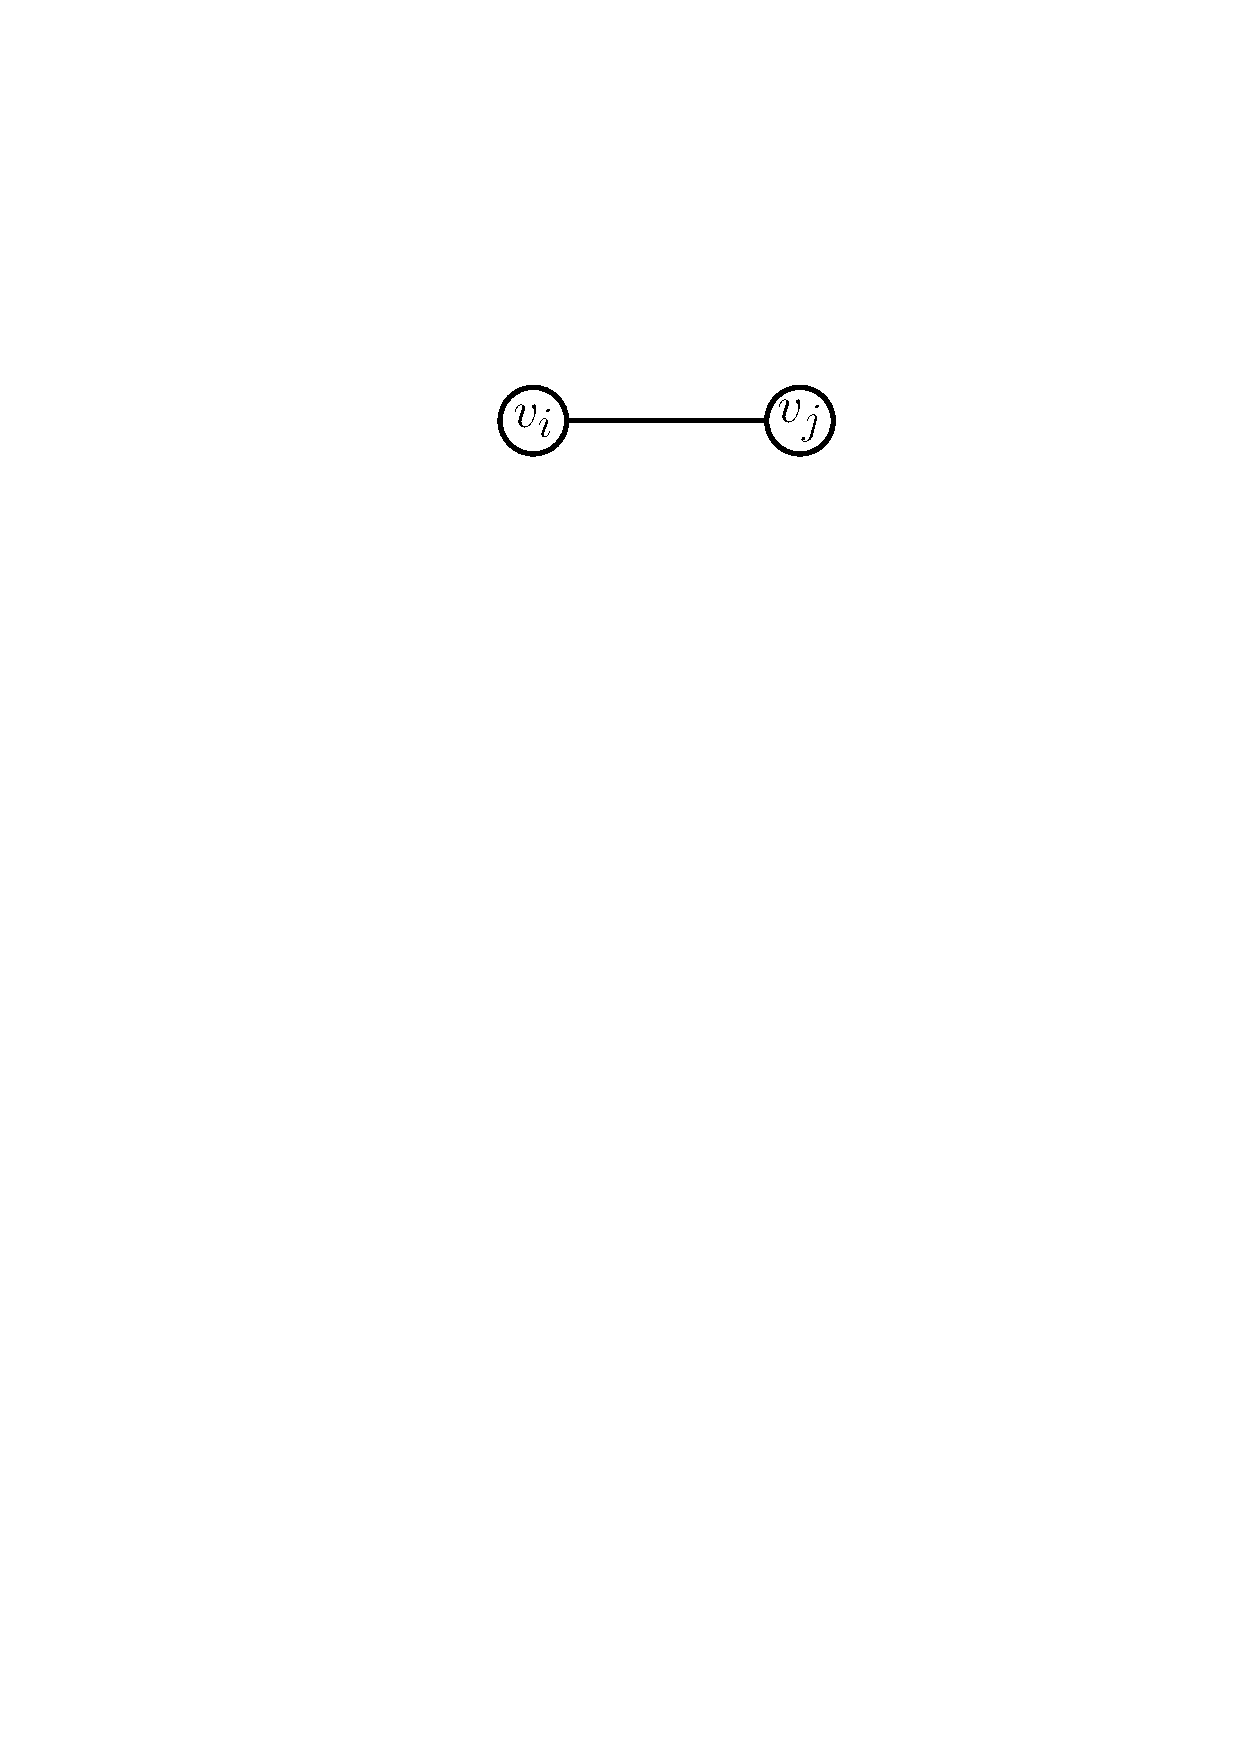
\includegraphics[scale=.5]{01_graph_theory/pics/adjacency_k-1.pdf}
}
\subfigure[adjacency $k = 2$]{
	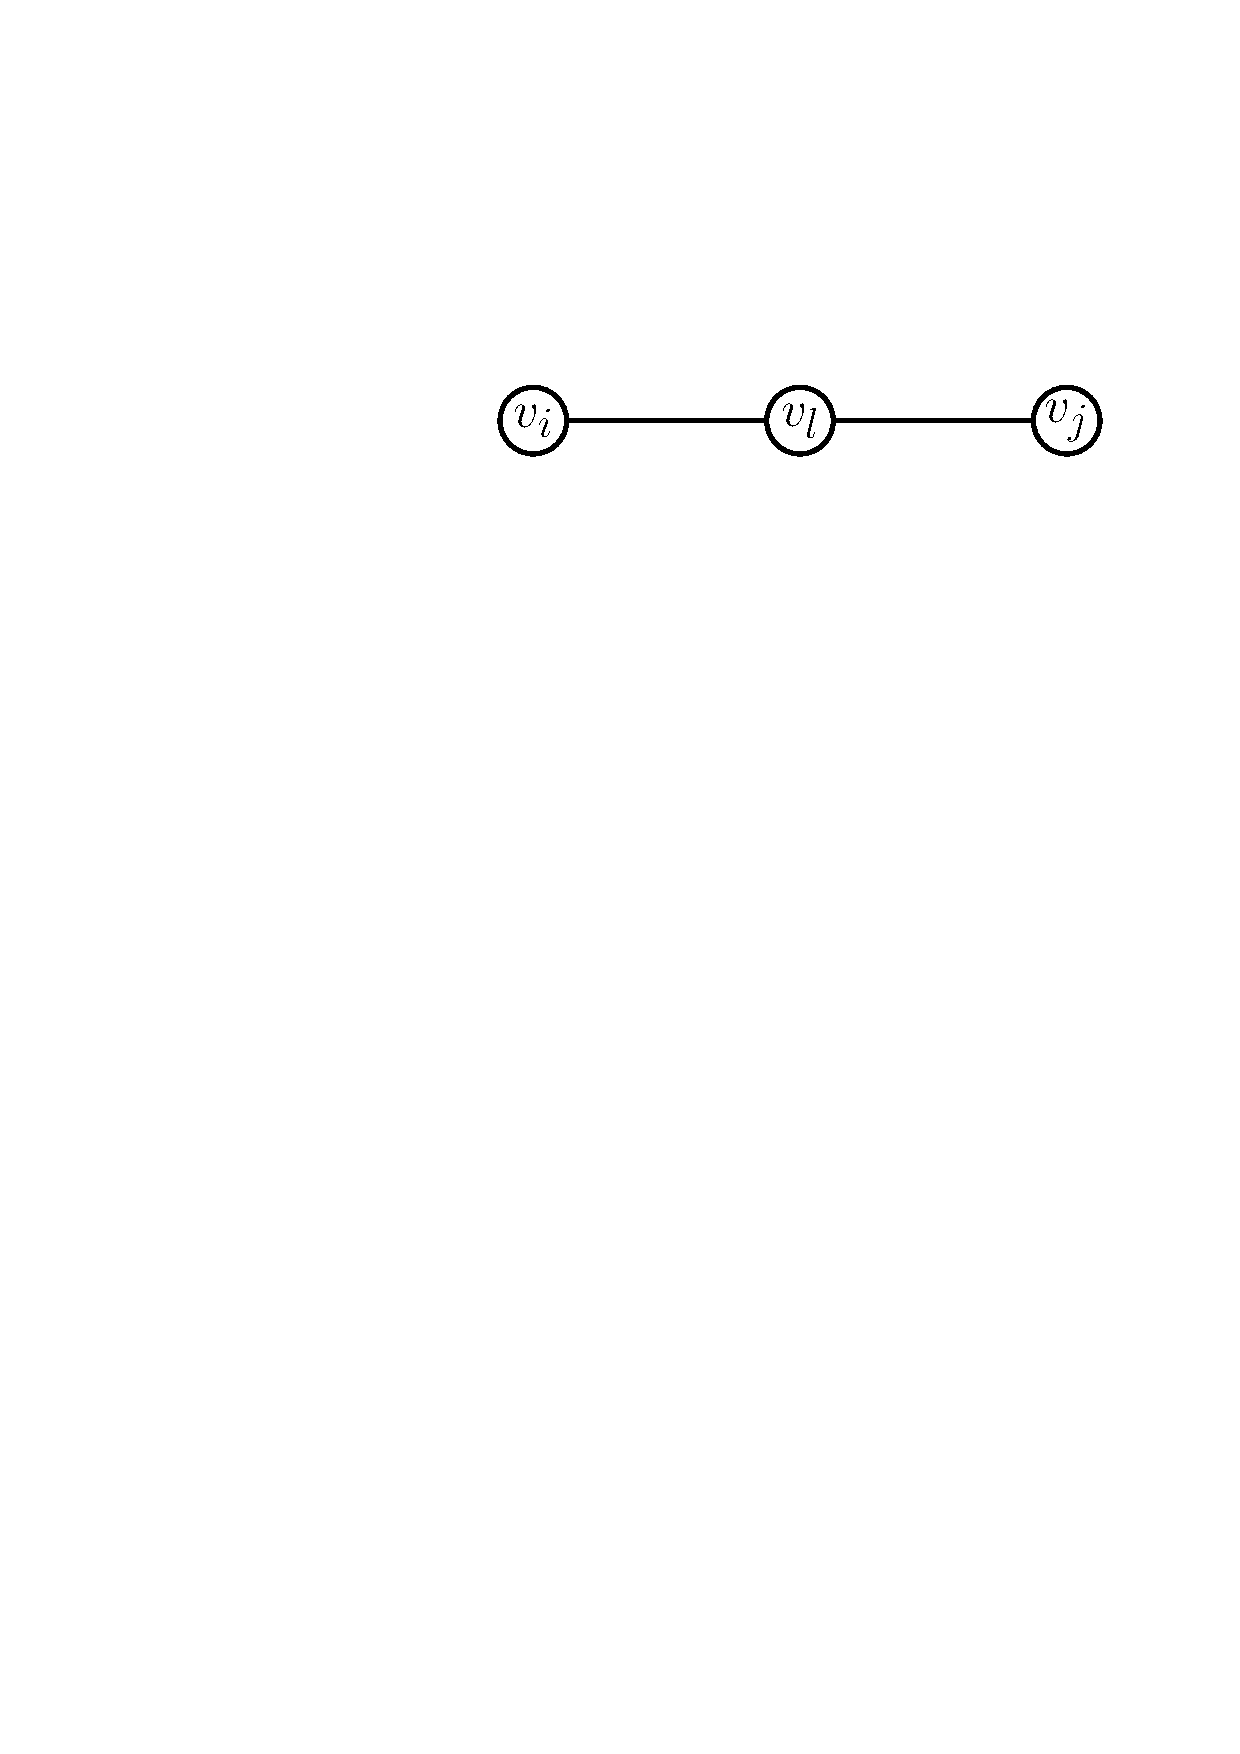
\includegraphics[scale=.5]{01_graph_theory/pics/adjacency_k-2.pdf}
}
\subfigure[adjacency via induction]{
	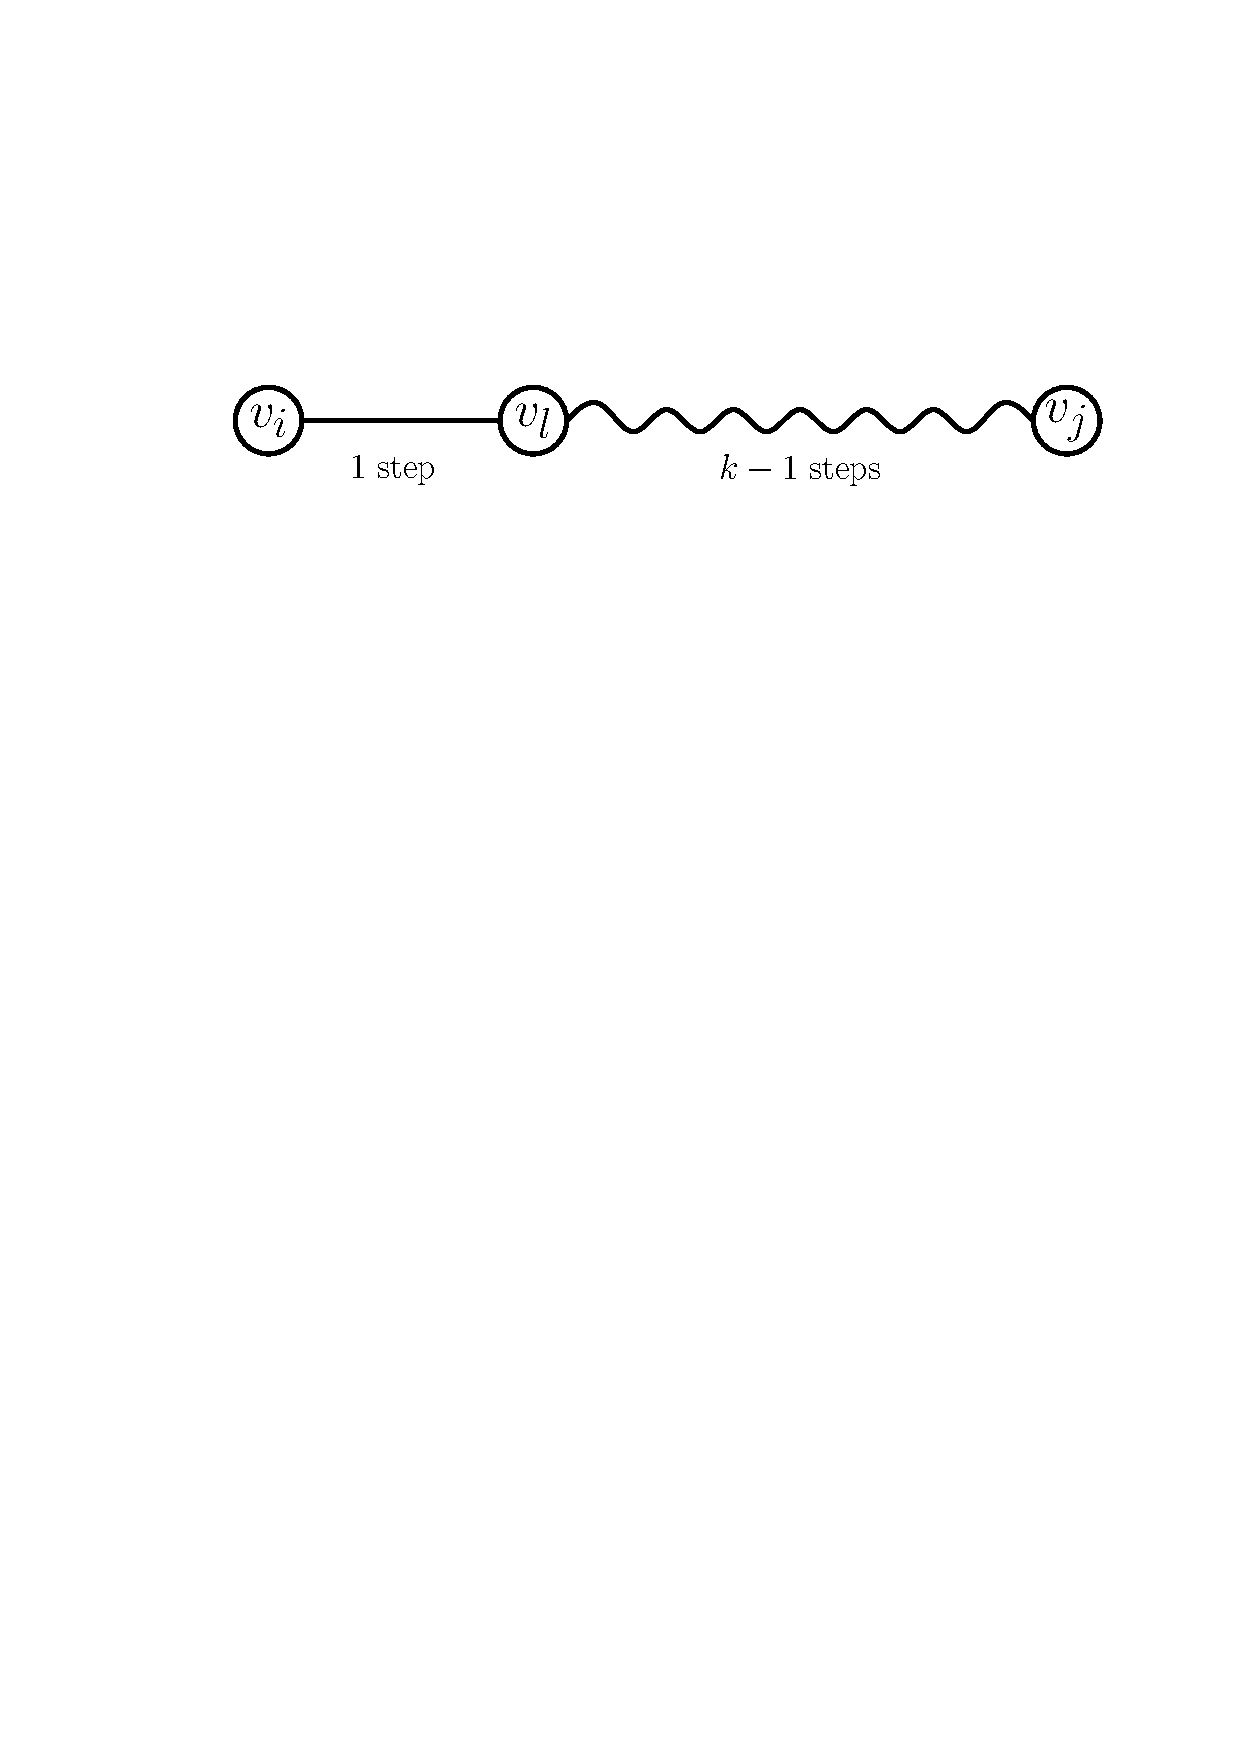
\includegraphics[scale=.5]{01_graph_theory/pics/adjacency_k-induction.pdf}
}
\caption{adjaceny}
\end{figure}
\FloatBarrier

\subsubsection*{Def:}
\begin{tabular}{l l}
Walk \\
	& 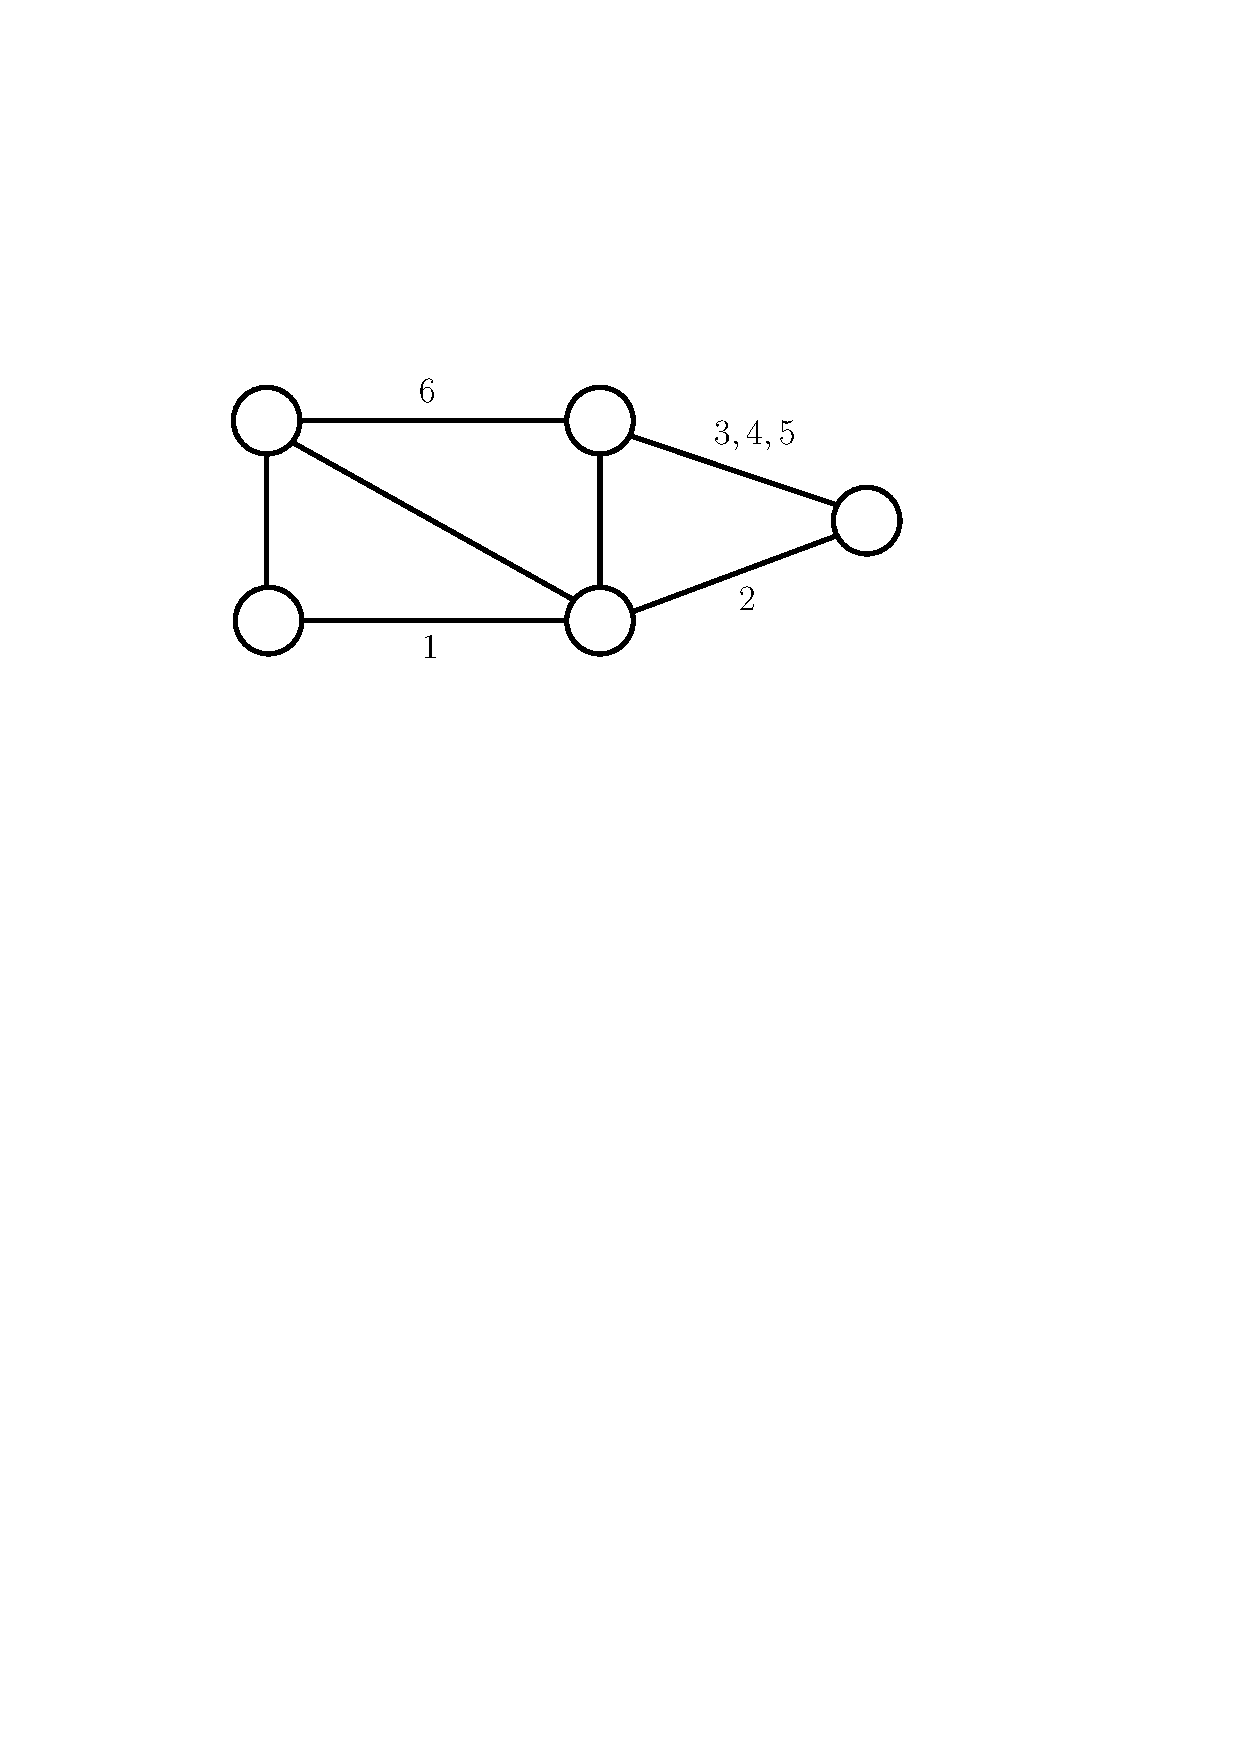
\includegraphics[scale=.5]{01_graph_theory/pics/walk.pdf}\\

Trail	& no edge repeated \\

closed trail	& = circuit \\

$G=(V,E)$ \\
Subgraph $ H = (V',E')$	& s.t. $V' \subseteq V$, $E' \subseteq E$ \\
$H \subseteq G$ \\

\end{tabular}

\vspace{12pt}

\begin{tabular}{l l}
$\sim$ : adjacent relation \\

v connected to w ($vRw$) \\

$C = \sum_{k=0}^L A ^k$ 	& $ L = min(|E|, |V| -1)$ \\
$C=(c_{ij}) $ \\
$C = $\# walks of length $\leq$ L, $v_i \leadsto v_j$ \\

$M = sign(C)$ (connectivity matrix\\

$\forall v \in V: vRv$ \\
$\forall v,w \in V: vRw = wRv$ & R \ldots equivalence relation\\
$\forall v,w,u \in V: vRw \cap wRu \Rightarrow vRu$ & $ \Rightarrow$ R induces Partition of V \\

\end{tabular}


\subsubsection*{Def:}
G is connected if $\forall v,w: vRw$

\subsubsection*{Def:}
$ H \leq G$  connected component of G if H connected, H maximal and connected
$V = V_1 \cap V_2 \cap \ldots \cap V_k$ \\
$V_i \ldots $ connected components of G

\begin{figure}[htb]
	\centering
	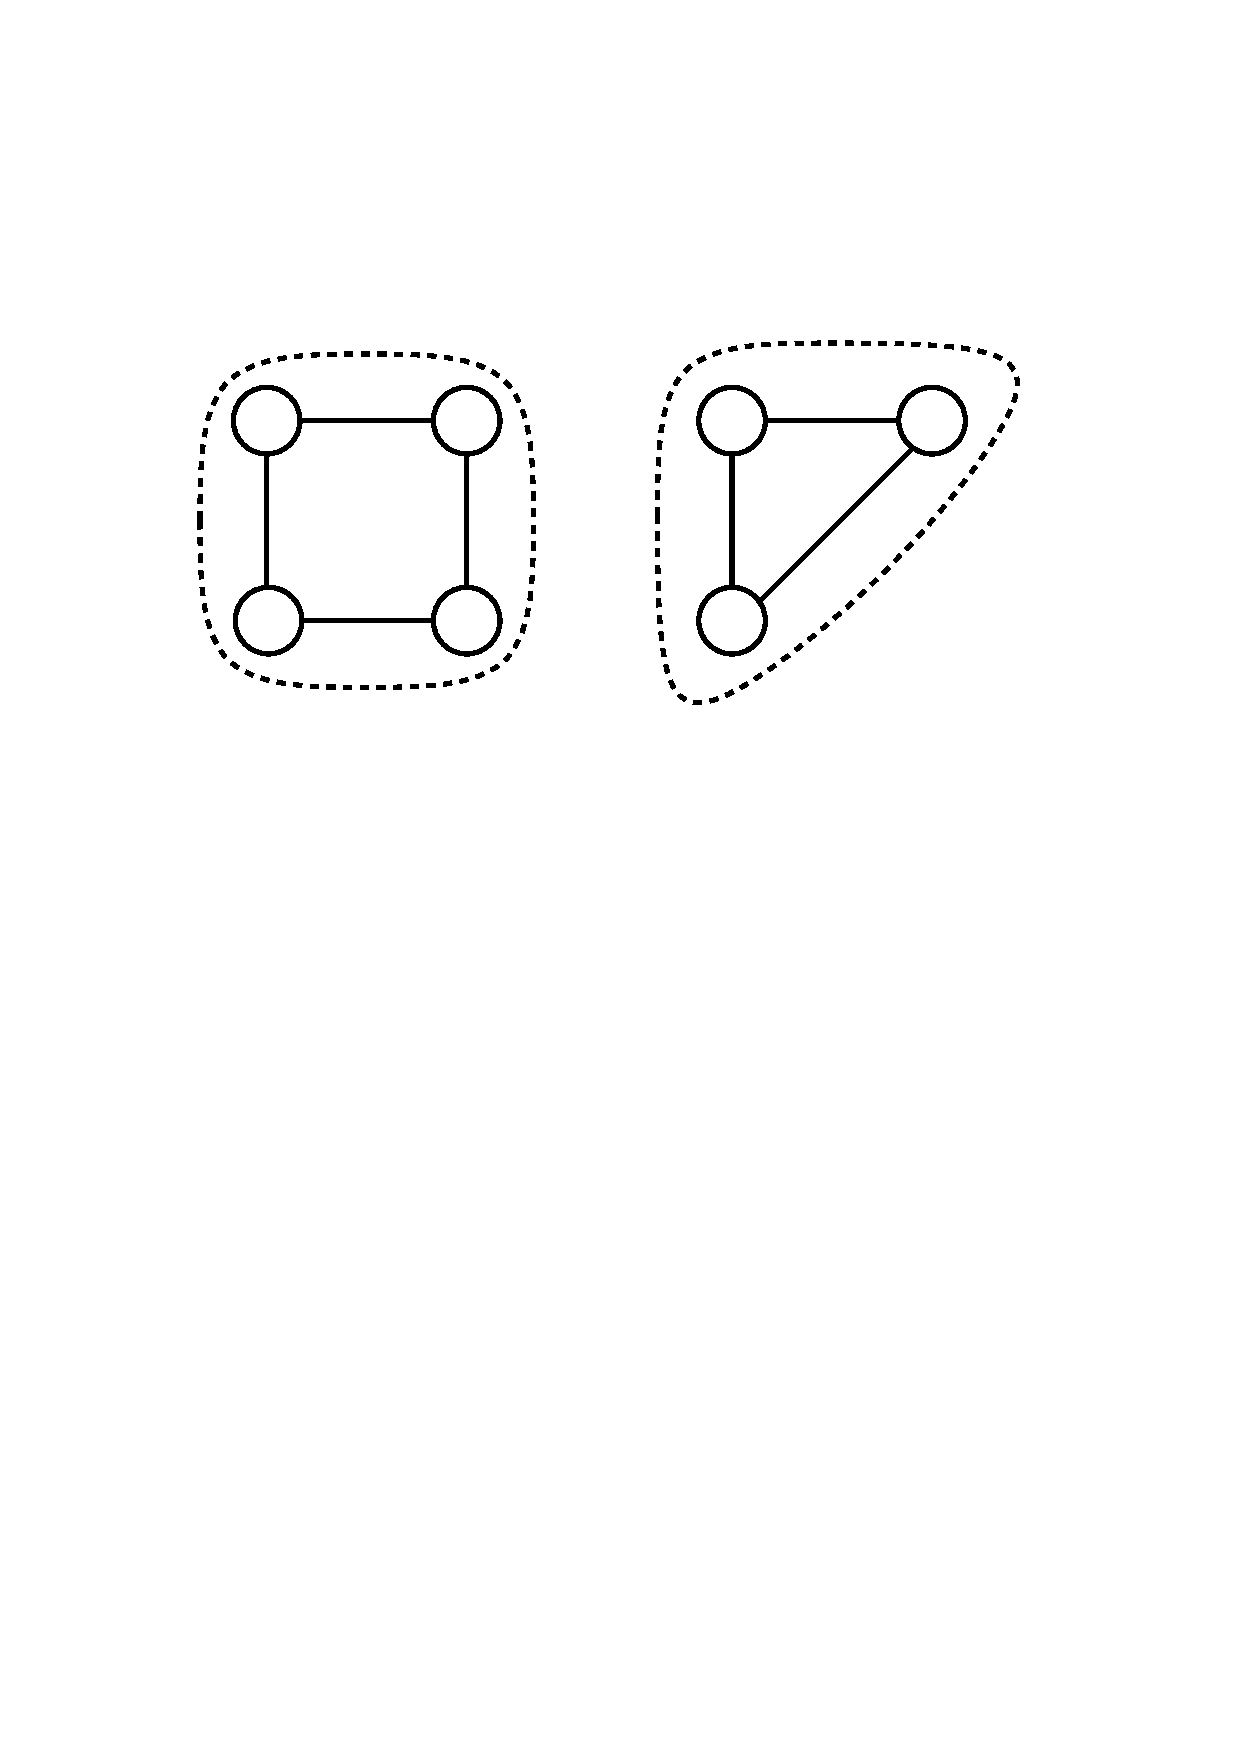
\includegraphics[scale=.5]{01_graph_theory/pics/components.pdf}
	\caption{Graph with 2 components}
\end{figure}
\FloatBarrier


\subsubsection*{$G$ directed}
$vSw : \implies \exists$ walk $v \leadsto w$ and walk from $w \leadsto v$

$S$ \ldots equivalent Relation $\Rightarrow$ $S$ induces a partition on $V$

\subsubsection*{Def:}
$G$ strongly connected $\implies \forall v,w \in V: vSw$ 


\subsection*{VO 02}

Directed Graph:

G strongly connected if $\forall vw : vSw$

$H \subseteq G: $ H strogly connected component if H max, str. con.

\subsubsection*{Rem:}
G strongly connected $\iff$ it has only 1 strongly connected component

G directed, H is the Graph G w/o (without) directions. then 
H \ldots shadow of G

G is weakly connected $\iff$ H connected

\begin{figure}[htb]
	\centering
	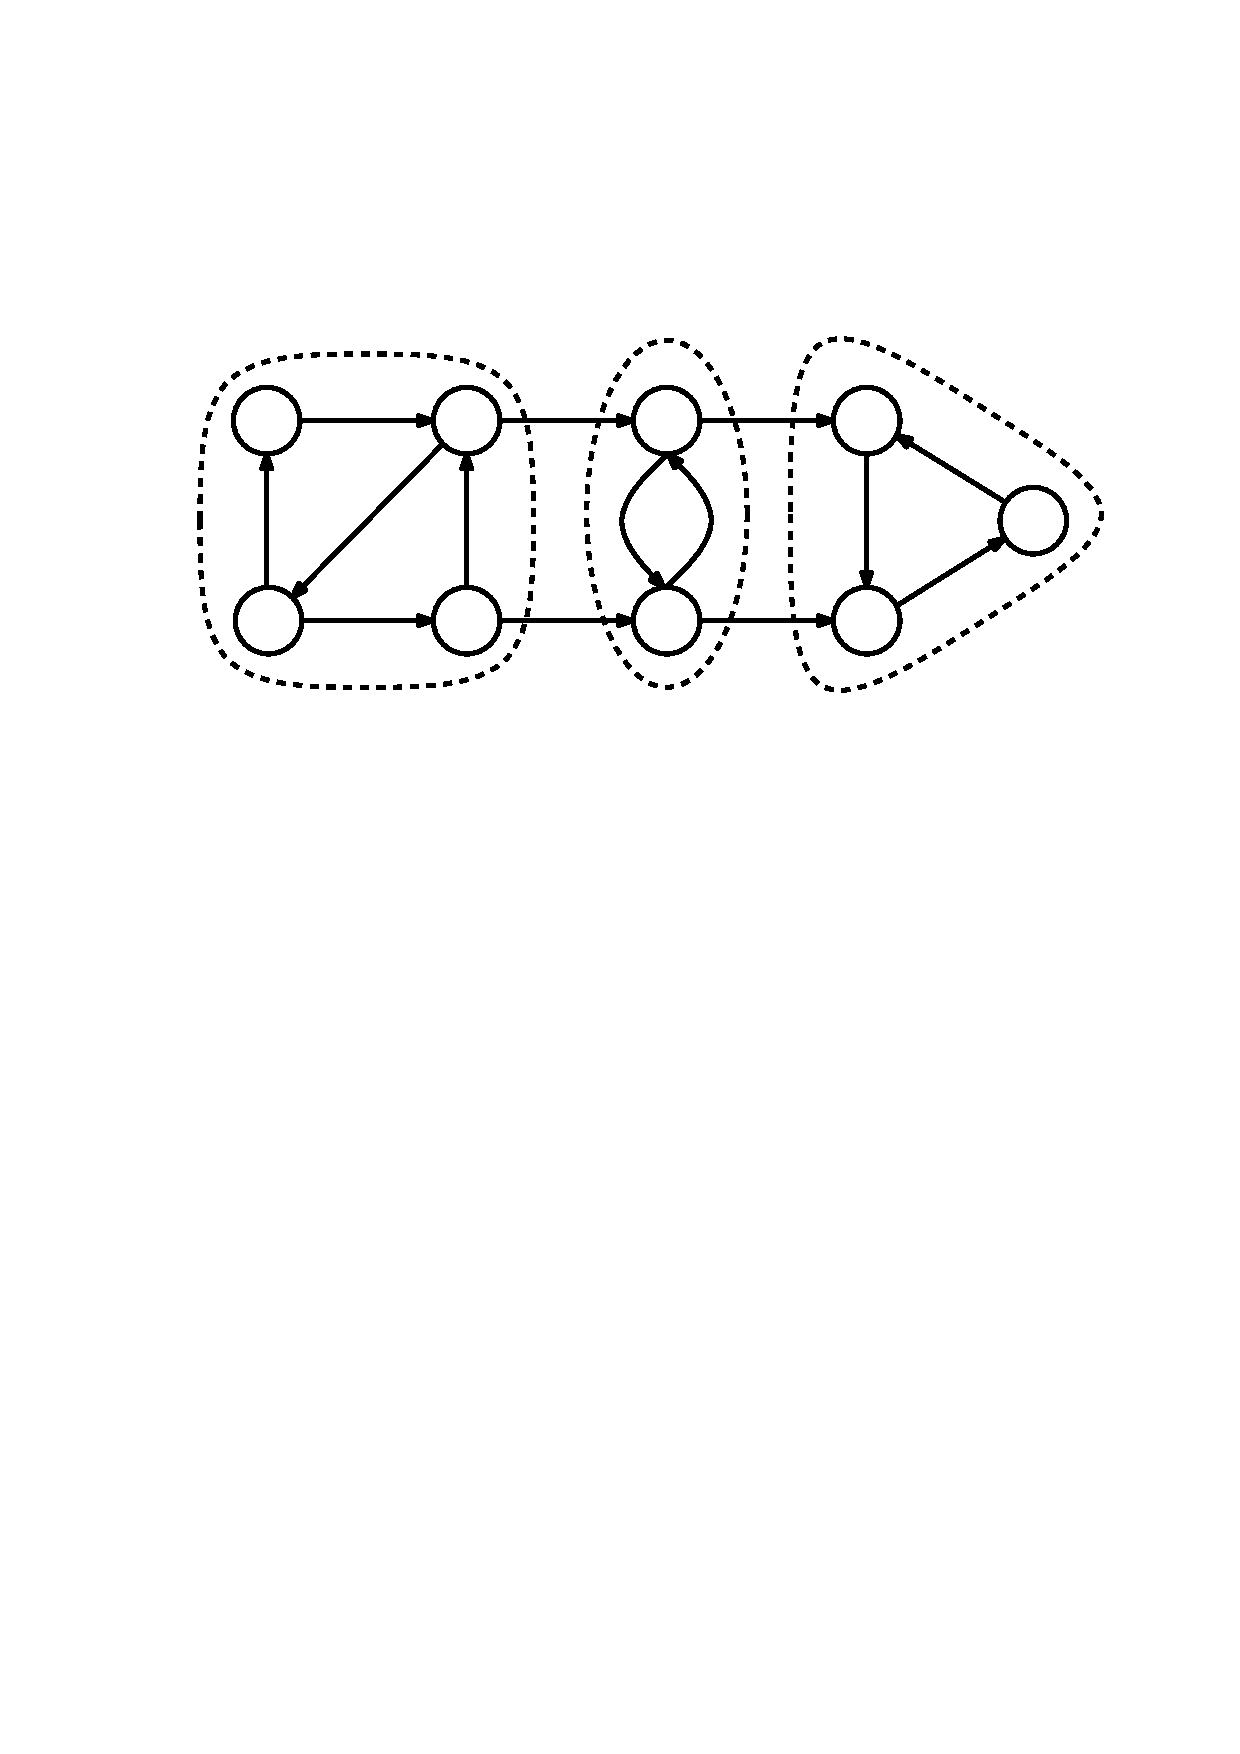
\includegraphics[scale=.5]{01_graph_theory/pics/strongly-connected_component.pdf}
	\caption{3 strongly connected components}
\end{figure}
\FloatBarrier

\subsubsection*{Def:}
$G$ directed, simple graph, 


$G_R = (V_R, E_R)$, reduction of $G$ \\
$V_R = \{K_1, K_2, \ldots , K_m\}$ set of str. con. comp. of $G$ \\
$E_r = \{ (K_i, K_j) | \exists v \in V(K_i) \exists w \in (K_j) : (v,w) \in E \}$

\subsubsection*{Rem:}
$G_R$ is always acyclic
$G$ strongly connected, then $G_R = ( \{ \bullet \}, \emptyset )$

\subsubsection*{Def: node base:}
$G=(V,E) $ directed, B \ldots node base, if:
\begin{enumerate}
\item $B \subseteq V$ 
\item $\forall v \in V \exists w \in B : wSv$
\item $B$ minimal w.r.t. $\subseteq$
\end{enumerate}

\subsubsection*{Rem: }
\begin{itemize}
\item node base of $G$ can be const from the node base of $G_R$ \\
	$\{K_1, \ldots , K_l\} $ node base of $G_R$ $\Rightarrow$ 
	$\{\{b_1, \ldots , b_l | b_i \in V(K_i)\}\}$ \ldots set of all node bases of $G$

\item node base of $G_R$ is $\{K \in V_R | d_{G_R}^{-}(K) = 0 \}$ of any acyclic graph
\end{itemize}
